\documentclass[10pt,a4paper]{article}
\usepackage[T1]{fontenc}
\usepackage[utf8]{inputenc}
\usepackage{amsmath, amssymb, amsthm, thmtools, amsfonts, mathtools}
\usepackage{nicefrac}
\usepackage{calc}
\usepackage[pdftex, hyperindex, plainpages=false]{hyperref}
\usepackage[nameinlink]{cleveref} %load before classicthesis (clash)
%\usepackage[nochapters,pdfspacing]{classicthesis}
\usepackage{siunitx}
\usepackage[siunitx]{circuitikz}

\usepackage[a4paper]{geometry}
\usepackage{float}
\usepackage{mdframed}
\usepackage{titling}
\usepackage{booktabs}
\usepackage{graphicx}
\usepackage{caption, subcaption}
\usepackage{xcolor}
\usepackage[italian]{babel}
\usepackage{pgfplots}
\usepackage{listings}
%\usepackage{lmodern}
\usepackage{url}
\usepackage{enumitem}
\usepackage{tikz} %loads after classicthesis (xcolor incompat)

% lets graphicx know path where figures to be included are found
\graphicspath{{../figs/}}
\makeatletter
\def\input@path{{../figs/}}
%or: \def\input@path{{/path/to/folder/}{/path/to/other/folder/}}
\makeatother

% tikz pgf plots setup
\usepgfplotslibrary{external}
\pgfplotsset{compat=1.15}
%\tikzexternalize

% spaces and significant digits/figures for measurements
\sisetup{free-standing-units, space-before-unit, number-unit-product = \;,
scientific-notation = false, round-mode = figures, round-precision = 1,}

% turns all (hyperlinked) references black [default is blue]
\hypersetup{
	linktoc=all,
	colorlinks=true,
	linkcolor=black
}

% code listings config
%\lstset{
%language=Python,
%basicstyle=\ttfamily,
%columns=fullflexible,
%keepspaces=true,
%}

% mdframed (for boxed text) configuration
\mdfsetup{linewidth=0.6pt}

% Default fixed font does not support bold face
\DeclareFixedFont{\ttb}{T1}{txtt}{bx}{n}{12} % for bold
\DeclareFixedFont{\ttm}{T1}{txtt}{m}{n}{12}  % for normal

% Custom colors
\usepackage{color}
\definecolor{deepblue}{rgb}{0,0,0.5}
\definecolor{deepred}{rgb}{0.6,0,0}
\definecolor{deepgreen}{rgb}{0,0.5,0}

% Commands 
\newcommand{\executeiffilenewer}[3]{%
	\ifnum\pdfstrcmp{\pdffilemoddate{#1}}%
		{\pdffilemoddate{#2}}>0%
	{\immediate\write18{#3}}\fi%
}
% input .svg --> .pdf_tex graphs
%\newcommand{\includesvg}[1]{%
%	\executeiffilenewer{#1.svg}{#1.pdf}%
%	{inkscape -z -D --file=#1.svg %
%	--export-pdf=#1.pdf --export-latex}%
%	\input{#1.pdf_tex}%
%}
% Thanks UniPi's Department of Physics E. Fermi
\newcommand{\thanksdf}{(\thanks{Dipartimento di Fisica E.~Fermi,%
Universit\`a di Pisa - Pisa, Italy.}\;)}

% hyperlink to email address
\newcommand{\mail}[1]{\href{mailto:#1}{\textsf{#1}}}

% \vec for bold vectors, instead of overarrows (now "\arrvec")
\let\arrvec=\vec
\renewcommand{\vec}[1]{\boldsymbol #1}
% replaces straight phi with slanted phi
\renewcommand{\phi}{\varphi}
% replaces straight eps with curved epsilon
\newcommand{\eps}{\varepsilon}
% abbreviation for (sub_/super^)scripts of \lim, \sum,... in inline math
\newcommand{\ds}{\displaystyle}

% blackboard/number set letters
\newcommand{\CC}{\mathbb C}
\newcommand{\HH}{\mathbb H}
\newcommand{\KK}{\mathbb K}
\newcommand{\NN}{\mathbb N}
\newcommand{\PP}{\mathbb P}
\newcommand{\QQ}{\mathbb Q}
\newcommand{\RR}{\mathbb R}
\newcommand{\ZZ}{\mathbb Z}

\newcommand{\Abs}[1]{{\left\Vert #1\right\Vert}}
\newcommand{\enclose}[1]{{\left( #1 \right)}}
\newcommand{\Enclose}[1]{{\left[ #1 \right]}}
\newcommand{\floor}[1]{\left\lfloor #1 \right\rfloor}
\newcommand{\ceil}[1]{\left\lceil #1 \right\rceil}
\newcommand{\To}{\rightrightarrows}

% Math operators
\DeclareMathOperator{\divergence}{div}
\renewcommand{\div}{\divergence}
\DeclareMathOperator{\Imaginarypart}{Im}
\renewcommand{\Im}{\Imaginarypart}
\DeclareMathOperator{\Realpart}{Re}
\renewcommand{\Re}{\Realpart}
%\DeclareMathOperator{\arg}{arg}
\DeclareMathOperator{\tg}{tg}
\DeclareMathOperator{\arctg}{arctg}
\DeclareMathOperator{\settsinh}{settsinh}
\DeclareMathOperator{\settcosh}{settcosh}
\DeclareMathOperator{\tr}{tr}
\DeclareMathOperator{\im}{im}
\DeclareMathOperator{\sgn}{sgn}
\DeclareMathOperator{\diag}{diag}

\DeclarePairedDelimiter{\norm}{\lVert}{\rVert}
\DeclarePairedDelimiter{\scalar}{\langle}{\rangle}

% Logarithm with arbitrary base.
% -> log_10
\newcommand{\llog}[1][10]{\log_{#1}}

% Absolute value.
% -> |x|
\newcommand{\abs}[1]{\left| #1 \right|}

% Powers.
% -> x^a
\newcommand{\power}[2][2]{\left( #2 \right)^{#1}}

% Square.
% -> x^2
\newcommand{\sq}[1]{\power[2]{#1}}

% Expansion of the binomial coefficient.
% -> n1!/(n2!(n1 - n2)!)
\newcommand{\binomexpr}[2]{\frac{#1!}{#2!(#1 - #2)!}}

% Expression evaluation at a given point with square brackets.
% -> [x]_{a}
\newcommand{\at}[2]{\left[ #1\right]_{\makebox[-1pt][l]{${\scriptstyle#2}$}}}

% Expression evaluation in an interval.
% -> [x] _{a}^{b}
\newcommand{\eval}[3]{\left.#1%
  \right|_{\makebox[-1pt][l]{${\scriptstyle#2}$}}^{\makebox[-1pt][l]{${\scriptstyle#3}$}}}

% Upright d in math mode (for differentials).
% -> d
\newcommand{\ud}{\mathrm{d}}

% Differential.
% -> dx
\newcommand{\diff}[1][x]{\,\ud{#1}}

% Base command for defining derivatives.
% -> df/dx or d^kf/dx^k
\newcommand{\basederivative}[4][]{%
  \displaystyle%
  \ifx\\#1\\\frac{#4#2}{#4#3}%
  \else%
  \frac{#4^#1#2}{#4#3^#1}%
  \fi%
}

% Total derivative.
% -> df/dx(x) or d^kf/dx^k(x)
\newcommand{\td}[4][]{%
  \basederivative[#1]{#2}{#3}{\ud}%
  \ifx\\#4\\%
  \else%
  \mkern-4mu\left(#4\right)%
  \fi%
}

% Partial derivative.
% -> df/dx(x) or d^kf/dx^k(x)
\newcommand{\pd}[4][]{%
  \basederivative[#1]{#2}{#3}{\partial}%
  \ifx\\#4\\%
  \else%
  \mkern-4mu\left(#4\right)%
  \fi%
}

\newcommand{\intinf}{\int_{-\infty}^{\infty}\!\!\!}

\newcommand{\cinterval}[2]{\left[\, #1,~#2 \,\right]}

\newcommand{\linterval}[2]{\left[\, #1,~#2 \,\right)}

\newcommand{\rinterval}[2]{\left(\, #1,~#2 \,\right]}

\newcommand{\ointerval}[2]{\left(\, #1,~#2 \,\right)}

\newcommand{\prob}[1]{\displaystyle P\left(#1\right)}

\newcommand{\pvalue}{\emph{$p$-value}}

\newcommand{\cond}{\,|\,}

\newcommand{\expect}[1]{\displaystyle E\left[#1\right]}

\newcommand{\mom}[2][]{\displaystyle {\cal M}_{#2}\ifx\\#1\\\else(#1)\fi}

\newcommand{\momalg}[1]{\displaystyle \lambda_{#1}}

\newcommand{\momcen}[1]{\displaystyle \mu_{#1}}

\newcommand{\skewness}{\displaystyle \gamma_1}

\newcommand{\kurtosis}{\displaystyle \gamma_2}

\newcommand{\charf}[1][x]{\phi_{#1}}

\newcommand{\momgenf}[1][x]{M_{#1}}

\newcommand{\fwhm}{{\scriptstyle \textsc{FWHM}}}

\newcommand{\hwhm}{{\scriptstyle \textsc{HWHM}}}

\newcommand{\median}{\mu_{\nicefrac{1}{2}}}

\newcommand{\var}[1]{\ensuremath{\text{Var}\left(#1\right)}}

\newcommand{\cov}[2]{\ensuremath{\text{Cov}\left(#1, #2\right)}}

\newcommand{\corr}[2]{\ensuremath{\text{Corr}\left(#1, #2\right)}}

\newcommand{\like}{\mathcal L}

\newcommand{\likelihood}[2][]{\like\ifx\\#2\\\else(#2\ifx\\#1\\\else;#1\fi)\fi}

\newcommand{\chisq}{\ensuremath{\chi^2}}

\newcommand{\chisquare}[2][]{\chisq\ifx\\#2\\\else(#2\ifx\\#1\\\else;#1\fi)\fi}

\newcommand{\loglikelihood}[2][]{\log\likelihood[#1]{#2}}

\newcommand{\pdf}[3][]{#2(#3\ifx\\#1\\\else;#1\fi)}

\newcommand{\binomialpdf}[2][]{\pdf[#1]{\mathcal B}{#2}}

\newcommand{\multinomialpdf}[2][]{\pdf[#1]{\mathcal M}{#2}}

\newcommand{\poissonpdf}[2][]{\pdf[#1]{\mathcal P}{#2}}

\newcommand{\uniformpdf}[2][]{\pdf[#1]{u}{#2}}

\newcommand{\exponentialpdf}[2][]{\pdf[#1]{\varepsilon}{#2}}

\newcommand{\gausspdf}[2][]{\pdf[#1]{N}{#2}}

\newcommand{\chisquarepdf}[2][]{\pdf[#1]{\wp}{#2}}

\newcommand{\cauchypdf}[2][]{\pdf[#1]{c}{#2}}

\newcommand{\erf}[1]{\ensuremath{\text{erf}\left(#1\right)}}

\newcommand{\dccases}[4][]{#2 \ifx\\#2\\\else=\fi %
  \begin{cases}
    \displaystyle #3 & \text{per variabili discrete}\\
    \displaystyle #4 & \text{per variabili continue}#1
  \end{cases}
}
% sub/super-scriptable for all symbol as math operator 
\newcommand\Scaleforall[1]{\vcenter{\hbox{\scalefont{#1}$\forall$}}}

\DeclareMathOperator*\forevery{%
  \vphantom\sum
  \mathchoice{\Scaleforall{2}}{\Scaleforall{1.4}}{\Scaleforall{1}}{\Scaleforall{0.75}}}
\geometry{left=2cm, right=2cm, top=2cm, bottom=2cm}

% indexes subsections with letters, sections with numbers (1.a, 1.b, ...)
\renewcommand{\thesubsection}{\thesection.\alph{subsection}}

% lets graphicx know path where figures to be included are found
\graphicspath{{../figs/}}

\author{Gruppo 1.AC \\ Matteo Rossi, Bernardo Tomelleri}
\title{Es05A: Applicazioni non-lineari di amplificatori operazionali}
\begin{document}
\date{\today}
\maketitle

\setcounter{section}{0}

\section*{Misura componenti dei circuiti}
\begin{table}[htbp]
\centering
\begin{tabular}{cccccc}
\toprule
Resistenze $[\si{k\ohm}]$ & $R$ & $\sigma R$ & Capacità $[\si{n\F}]$ & $C$ &
$\sigma C$ \\
\midrule
\midrule
$R_1^Q$	  & 100.6 	& 0.8 	 & $C_T$ & 1.00		 & 0.04 \\
$R_1^T$	  & 9.94	& 0.08 	 & $C_F$ & 1.00		 & 0.04 \\
$R_2^T$	  & 2.19	& 0.03	 & $C_1$ & 96		 & 4	\\
$R_2^a$	  & 9.94	& 0.08	 & $C_2$ & 1.00		 & 0.04 \\
$R_3$	  & 9.92	& 0.08	 & & & \\
$R_4$	  & 9.94	& 0.08	 & & & \\
\bottomrule     
\end{tabular}
\caption{Valori di resistenza e capacità misurate per i componenti dei
circuiti studiati. \label{tab: rcmes_B}}

\begin{tabular}{cccccc}
\toprule
Resistenze $[\si{\ohm}]$ & $R$ & $\sigma R$ & Capacità $[\si{n\F}]$ & $C$ &
$\sigma C$ \\
\midrule
\midrule
$R_1^Q$	  & 99.8 	& 0.8 	 & $C_T$ & 1.00		 & 0.04 \\
$R_1^T$	  & 9.94	& 0.08 	 & $C_F$ & 1.00		 & 0.04 \\
$R_2^T$	  & 2.19	& 0.03	 & $C_1$ & 99		 & 4	\\
$R_2^A$	  & 9.87		& 0.08		 & $C_2$ & 1.00		 & 0.04 \\
$R_3^A$	  & 10.01		& 0.08		 & & & \\
$R_4^M$	  & 9.91		& 0.08		 & & & \\
\bottomrule     
\end{tabular}
\caption{Valori di resistenza e capacità misurate per i componenti dei
circuiti studiati. \label{tab: rcmes_M}}
\end{table}

Riportiamo per completezza anche i valori delle tensioni di alimentazione
continue per l'op-amp misurate con il multimetro
\begin{align*}
V_{CC} &= 4.99 \pm 0.03 \si{\V} \\
V_{EE} &= -4.99 \pm 0.03 \si{\V}
\end{align*}

Non è stato facile misurare i valori di capacità dei condensatori nel
circuito con il multimetro, che a volte con i soli puntali collegati legge
un rumore di fondo intorno ai $7 \pm 1 \; \si{n\F}$, abbastanza alto da
saturare il fondo scala da $\SI{2}{n\F}$ con cui si vorrebbero misurare i
valori delle capacità $C_T$, $C_F$ e $C_2$.

Per tutto il resto della trattazione come ampiezze dei segnali si intendono
misurate non ``picco - picco'', a meno che non venga esplicitato altrimenti.

\subsection*{Nota sul metodo di fit}
Per determinare i parametri ottimali e le rispettive covarianze si \`e
implementato in \verb+Python+ un algoritmo di fit basato sui minimi quadrati
mediante la funzione \emph{curve\_fit} della libreria \texttt{SciPy}.

%=======================
\section{Circuito amplificatore di carica}
\subsection{Progettazione del circuito}
Si è costruito un amplificatore di carica a partire da un op-amp TL081CP come
quello in figura \ref{fig: Qampschm}

\begin{figure}[htbp]
    \centering
	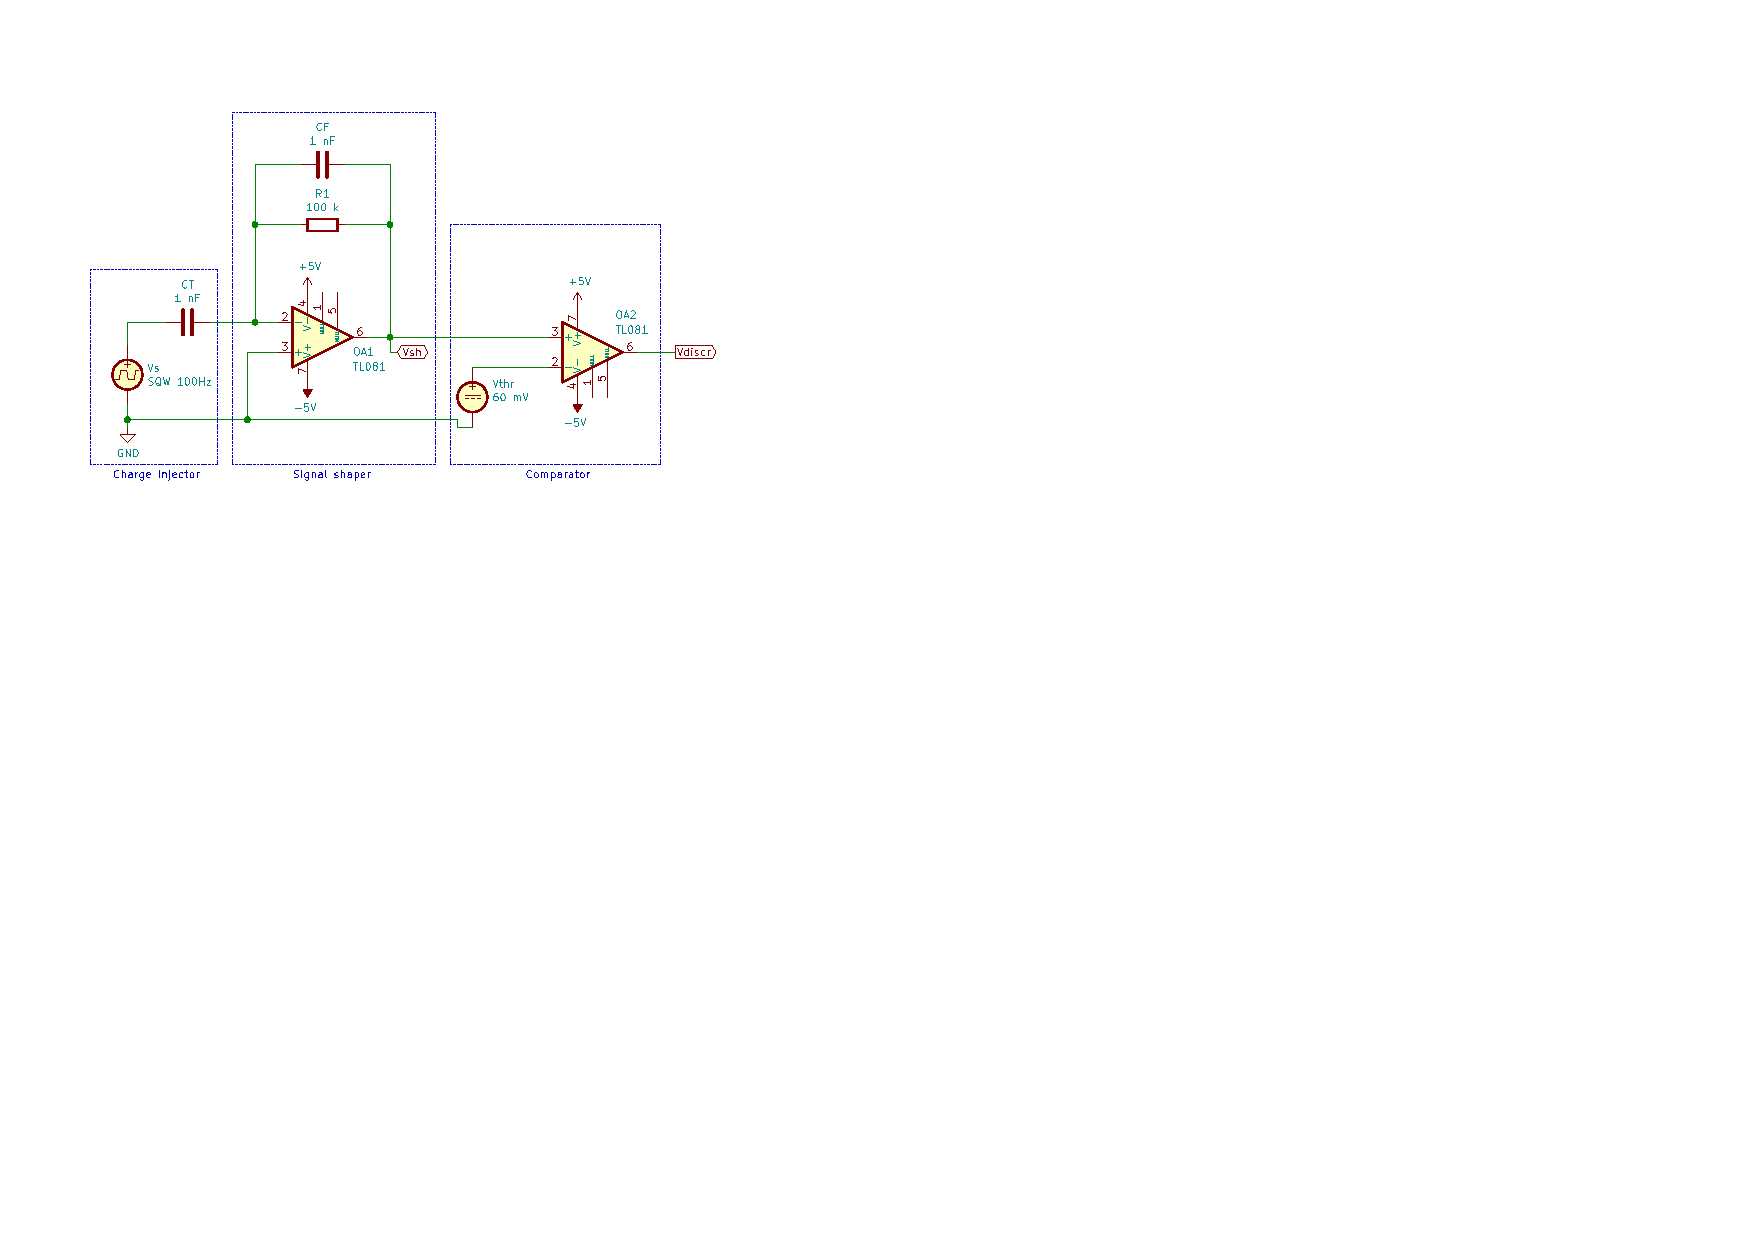
\includegraphics[scale=1.2]{Qamp}
    \caption{Schema circuitale dell'amplificatore di carica costruito.
    \label{fig: Qampschm}}
\end{figure}

In cui abbiamo indicato i sotto-circuiti di cui è composto, da sinistra verso
destra come: ``iniettore/rivelatore di carica'', ``circuito formatore/shaper''
(passa-basso/integratore attivo) e ``discriminatore/comparatore''.

\subsection{Funzionamento di iniettore e shaper}
Si è inviato all'ingresso di entrambi i circuiti un'onda quadra di
ampiezza $V_s = 999 \pm 8 \si{m\V}$ e frequenza fissata a
$f = 100.0 \pm 1.6 \; \si{\Hz}$, che corrisponde ad una carica
$Q\ped{in} = C_T \cdot 2V_s = 1.98 \pm 0.08 \; \si{n\coulomb}$, proporzionale
al ``salto'' di tensione dal livello alto a basso (e viceversa) dell'onda,
più semplicemente alla sua ampiezza picco-picco
$V_s^{pp} = 2 V_s \implies Q\ped{in} = C_T \cdot V_s^{pp}$.

Dunque abbiamo trovato come segnale in uscita dal circuito formatore un
segnale che dopo un breve transiente diventa un esponenziale decrescente,
con ampiezza iniziale $V\ped{sh} (t=0) = 2007 \pm 18 \; \si{m\V}$ e
con la stessa frequenza $99.9 \pm 1.6 \; \si{\Hz}$ dell'onda quadra.
Riportiamo in figura l'immagine acquisita dall'oscilloscopio con dettaglio
sul transiente al fronte di discesa dell'onda quadra.
\begin{figure}[htbp]
    \centering
	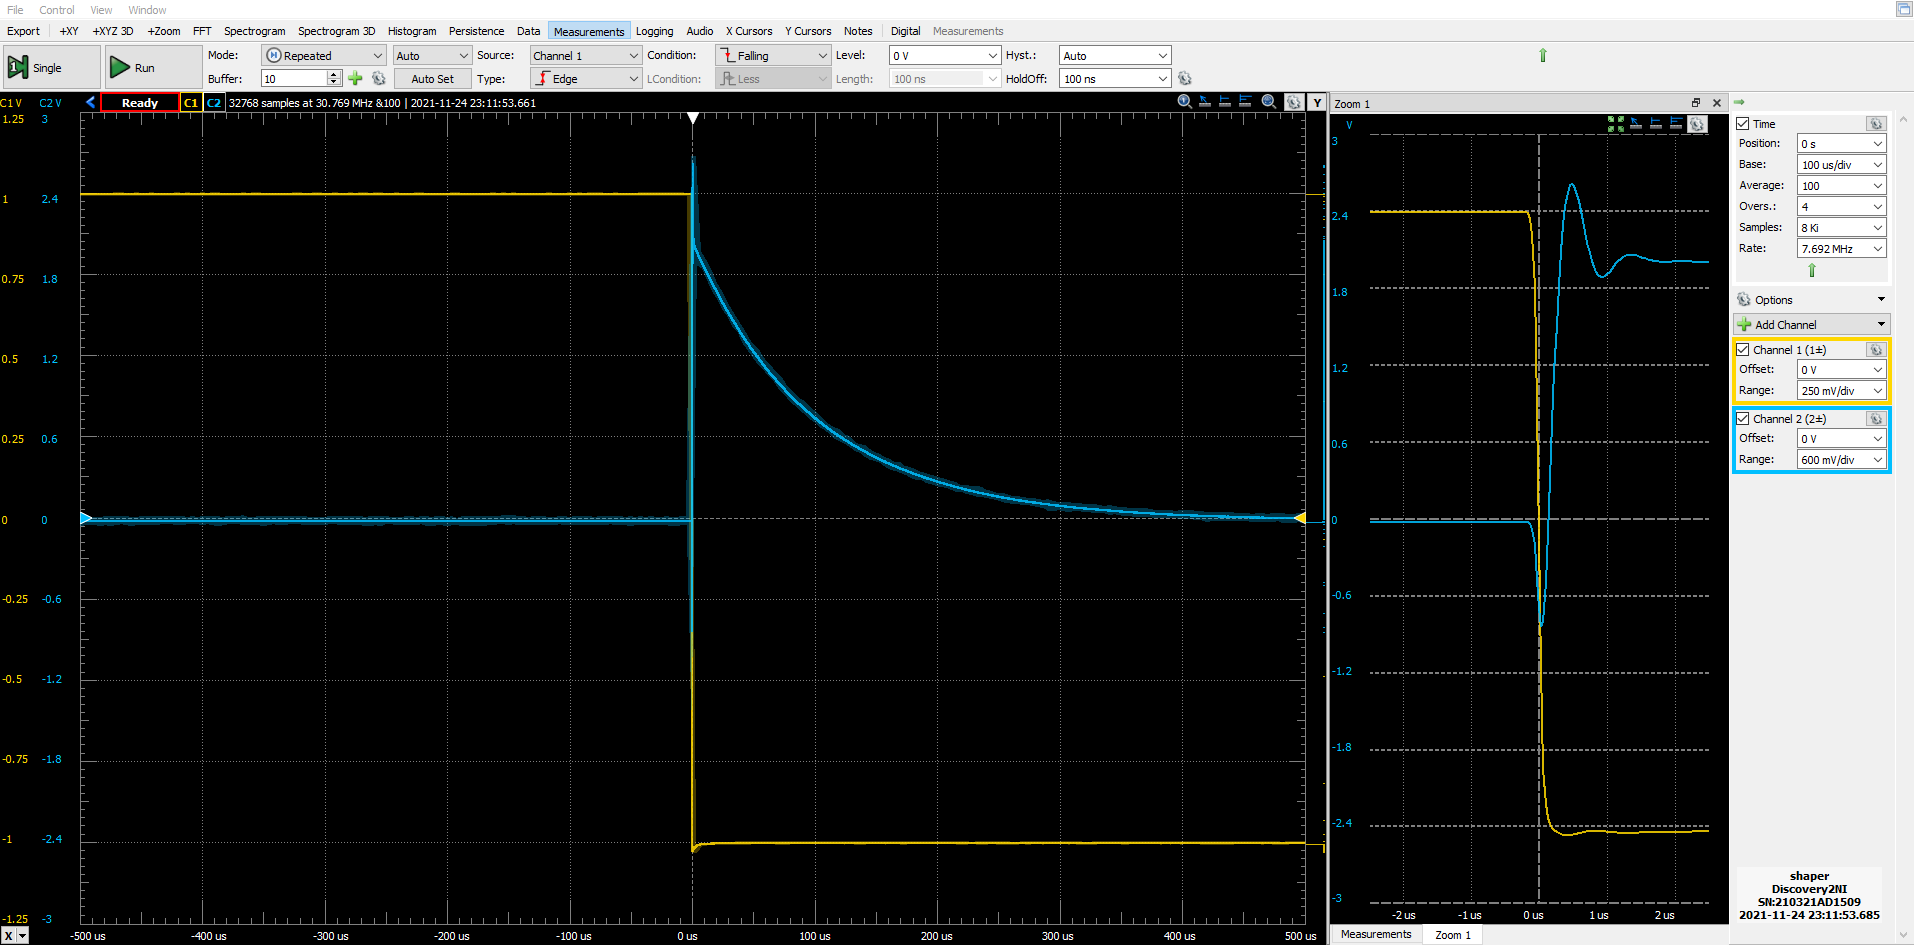
\includegraphics[scale=0.335]{shaperzoom}
    \caption{Acquisizione del segnale in uscita dal circuito formatore con
    un'onda quadra in ingresso $V_s = \SI{1}{V}$, $f= \SI{100}{\Hz}$
    \label{fig: shzoom}}
\end{figure}

Assumendo iniezione di carica istantanea sulle armature dei condensatori $C_T$
e $C_F$, il segnale in uscita dal sotto-circuito formato da $C_T$ e dal
formatore è legato al segnale in ingresso dalla relazione
\begin{align}\label{eq:Vsh}
V\ped{sh}(t) &= \frac{Q\ped{in}}{C_F} e^{-t/\tau} =
2V_s(t) \frac{C_T}{C_F} e^{-t/\tau} \\
\tau &= R_1 C_F
\end{align}
Per i circuiti in esame i valori delle capacità sono
$C_T \approx C_F = \SI{1}{n\F}$ e $R_1 = \SI{100}{\kilo\ohm}$,
per cui possiamo semplificare il rapporto $C_T/C_F \approx 1$, da cui
ricaviamo come valori attesi
\begin{align*}
V\ped{sh}(t) &= 2V_s(t) e^{-t/\tau} \\
\tau &= R_1 C_F = 100 \pm 4 \; \si{\micro\s}
\end{align*}
Quindi complessivamente come tensione in uscita $V\ped{sh} (t)$ ci aspettiamo
di osservare una serie di picchi seguiti da decrescite esponenziali di segno
alternante con l'onda quadra in ingresso e di ampiezza doppia.

Questo risulta compatibile con quanto si è osservato dall'oscilloscopio, che
riportiamo per chiarezza in figura~\ref{fig: shaper}
\begin{figure}[htbp]
    \centering
	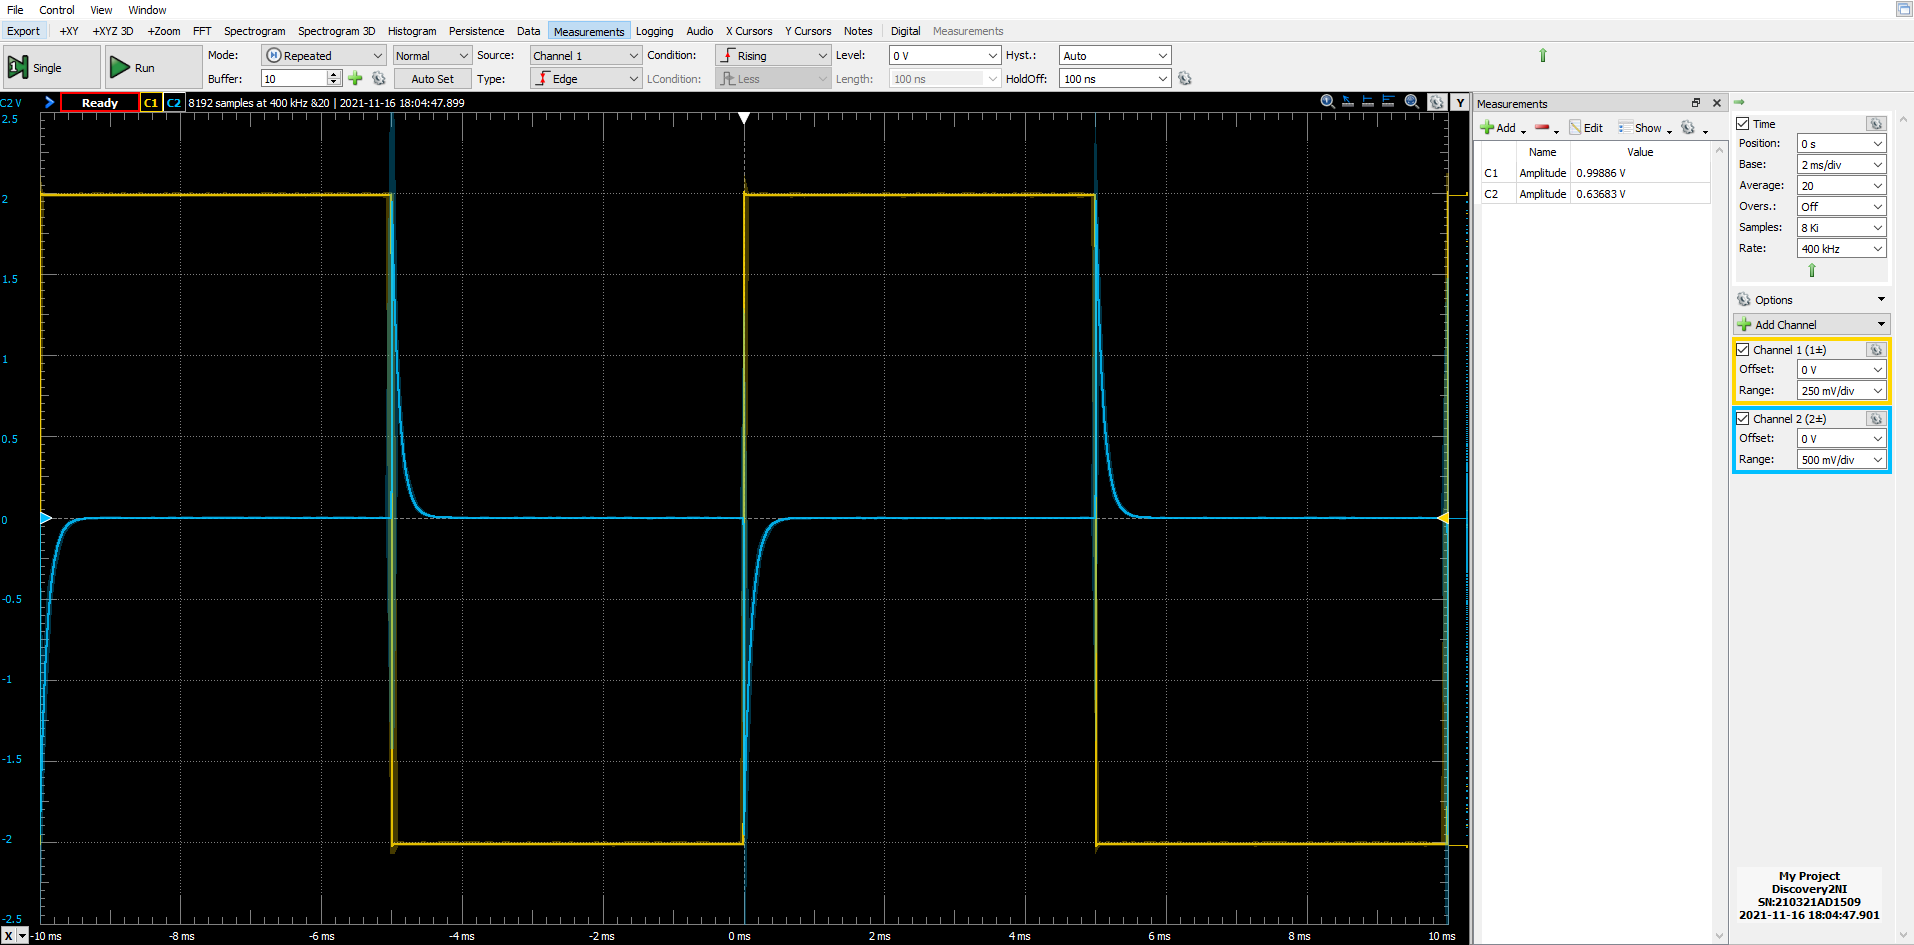
\includegraphics[scale=0.335]{shaper}
    \caption{Onda quadra in ingresso $V_s = \SI{1}{V}$, $f = \SI{100}{\Hz}$
    su CH1 e segnale in uscita dal circuito formatore $V\ped{sh}$ su CH2.
    \label{fig: shaper}}
\end{figure}

Dunque possiamo controllare che la forma d'onda esponenziale sia compatibile
con quanto atteso dalla \eqref{eq:Vsh} tramite un fit ai punti campionati
dall'AD2, di cui riportiamo brevemente i risultati
\begin{figure}[htbp]
    \centering
	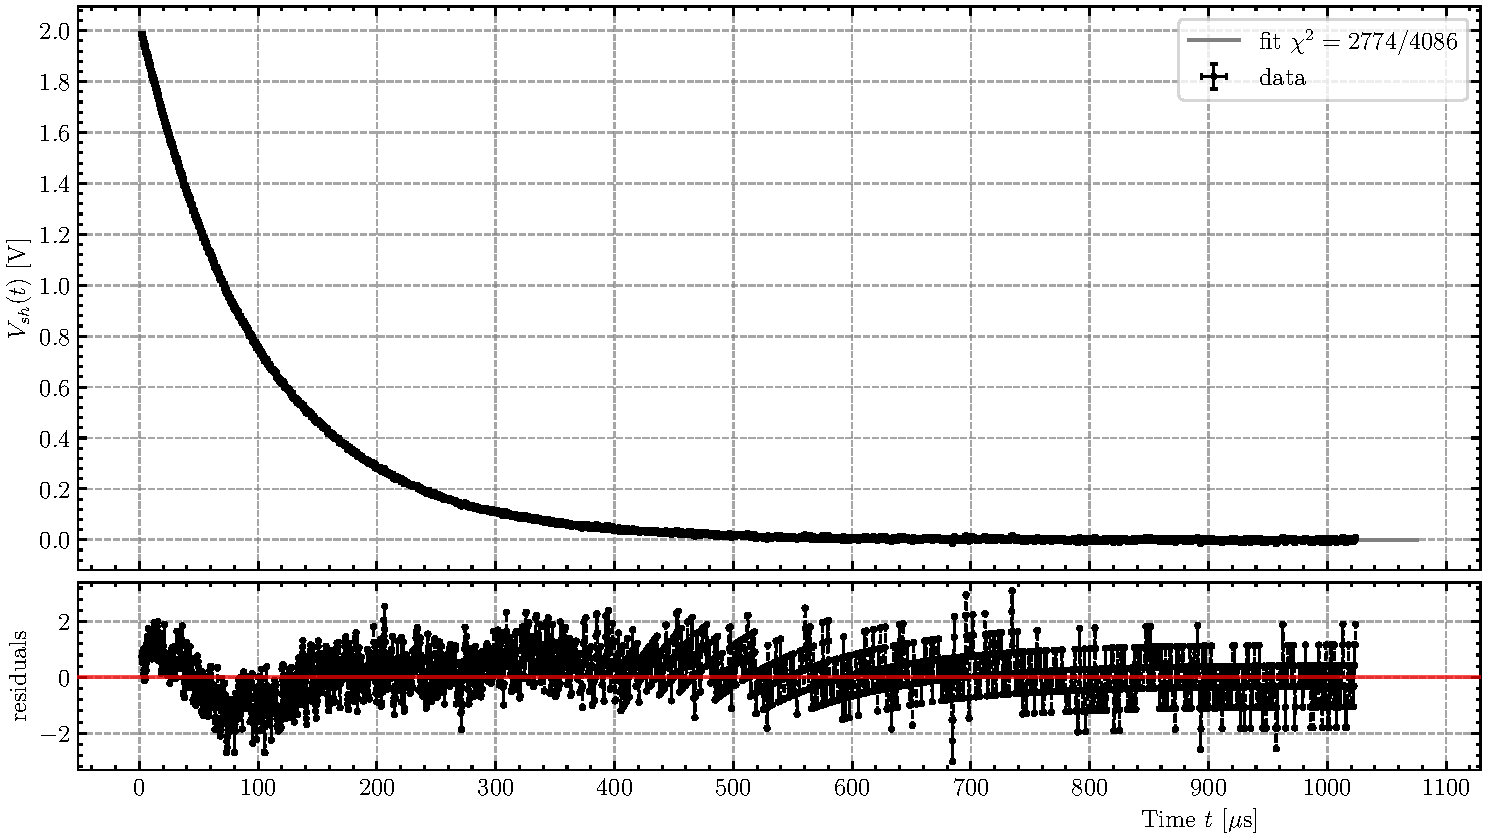
\includegraphics[scale=0.6]{tau}
    \caption{Fit con esponenziale decrescente al segnale in uscita dal
    circuito formatore $V\ped{sh}$ \label{fig: tau}}
\end{figure}
\begin{align*}
V\ped{sh} (t=0) &= 2021 \pm 2 \; \si{m\V}
&\tau = 101.88 \pm 0.03 \; \si{\micro\s} \\
\chi^2/\mathrm{ndof} &= 2774/4086 &\mathrm{cov_{norm}} = -0.75
\end{align*}

Da cui vediamo come non solo la misura di ampiezza iniziale sia compatibile
con il valore misurato, ma anche il tempo caratteristico di smorzamento $\tau$
risulta pienamente in accordo con il valore atteso dai componenti del
circuito.

\setcounter{subsection}{3}
\subsection{Funzionamento del discriminatore}
Il sotto-circuito discriminatore è un comparatore con tensione di soglia
misurata con l'oscilloscopio $V\ped{thr} = 51.9 \pm 0.4 \si{m\V}$ e fornita
dal generatore di tensione (con valore nominale $\SI{60}{m\V}$) \verb+W2+
collegato all'ingresso invertente del secondo OpAmp.

Supponiamo di essere sempre in regime di saturazione per l'OpAmp ideale e
come prima assumiamo iniezione istantanea di carica sui condensatori. 
Grazie al fatto che le tensioni di alimentazione sono pari in modulo
$V_{CC} = - V_{EE}$ possiamo prendere come segnale atteso in uscita
\begin{equation}\label{eq: Vdiscr}
V\ped{discr} (t) = V_{CC} \sgn\left[V\ped{sh}(t) - V\ped{thr}\right].
\end{equation}

Più esplicitamente, ricordando che $V\ped{sh}$ ha ampiezza (iniziale) doppia
rispetto all'ampiezza in ingresso $V_s$ (o proporzionale a $V_s^{pp}$)
\begin{itemize}
\item se $V_s^{pp} < V\ped{thr} \implies V\ped{discr} = V_{EE}$ costante.
\item se $V_s^{pp} \geq V\ped{thr}$, ci aspettiamo (in un periodo dell'onda
quadra di durata $T = 9.99 \pm 0.16 \; \si{m\s}$)
\[
V\ped{discr}(t) =
\begin{cases}
V_{CC} & 0 < t < ToT \\
V_{EE} & ToT < t < T
\end{cases}
\]
In cui $ToT$ è il tempo in cui il picco esponenzialmente decrescente è
maggiore della tensione di soglia
$V\ped{sh}(t) = \frac{Q\ped{in}}{C_F} e^{-t/\tau} \geq V\ped{thr}$, appunto il
``Time-over-Threshold''.
\begin{equation} \label{eq:ToT}
ToT = \tau \log\left(\frac{Q\ped{in}}{C_F V\ped{thr}}\right) =
\tau \log\left(\frac{C_T V_s^{pp}}{C_F V\ped{thr}}\right) = 
\tau \log\left(\frac{C_T}{C_F} \frac{2 V_s}{V\ped{thr}}\right).
  \end{equation}
\end{itemize}

Mantenendo lo stesso segnale in ingresso al circuito del punto precedente
(con ampiezza ben oltre la soglia $V_s \gg V\ped{thr}$) riportiamo il
segnale visualizzato all'oscilloscopio in uscita dal discriminatore in figura
\ref{fig: discr}.
\begin{figure}[htbp]
\centering
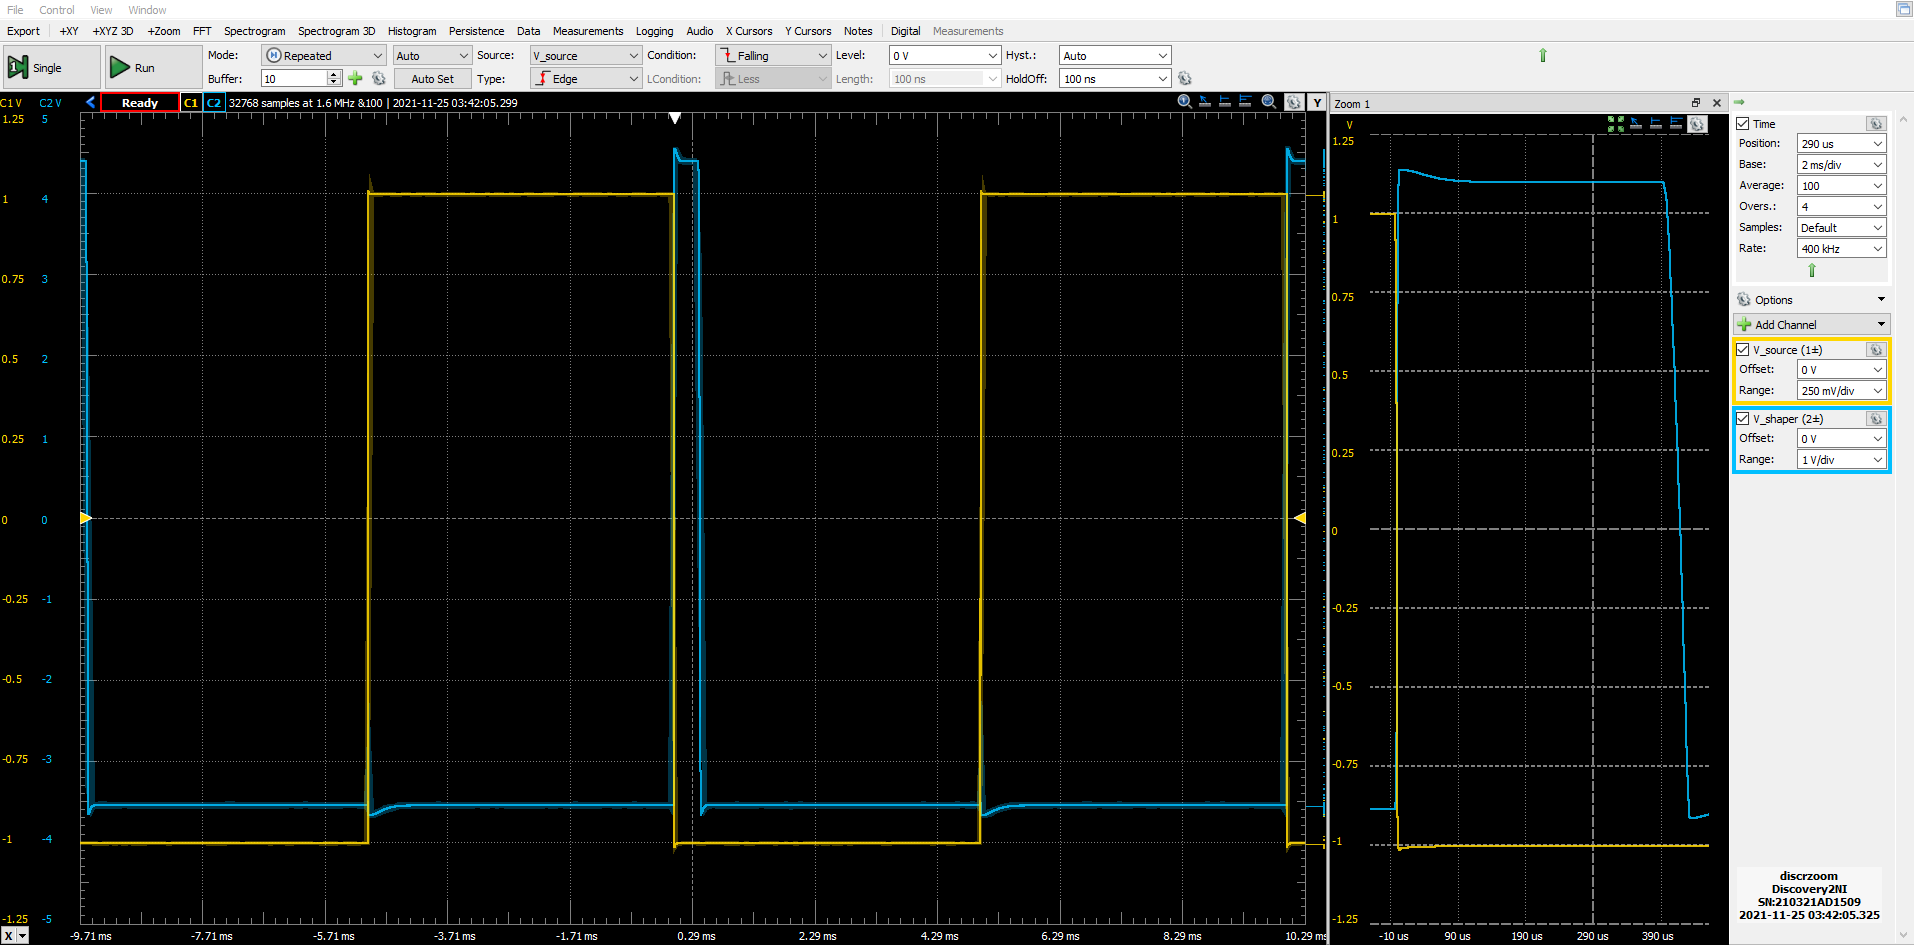
\includegraphics[scale=0.335]{discrzoom}
\caption{Acquisizione del segnale in uscita dal circuito comparatore con
un'onda quadra in ingresso $V_s = \SI{1}{V}$, $f = \SI{100}{\Hz}$
\label{fig: discr}}
\end{figure}

Risulta già chiaro dal dettaglio a destra, in corrispondenza del fronte di
discesa dell'onda quadra, come il segnale in uscita non abbia né livelli basso
e alto simmetrici rispetto a $\SI{0}{V}$, né pendenza uguale (idealmente
infinita) nel passaggio tra questi due, al contrario di quanto atteso dal
nostro modello semplificato.

Possiamo caratterizzare il segnale $V\ped{discr} (t)$ trovato come un impulso
di tensione con livello basso $V_{OL}$ e livello alto $V_{OH}$ di durata
$T_{OH}$ che si ripete periodicamente con la stessa frequenza dell'onda quadra
in ingresso $V_s (t)$.
Riportiamo le misure dirette effettuate con i cursori
delle tensioni di saturazione del comparatore e una misura del tempo ``alto''
dell'impulso definita in maniera compatibile con la funzione automatica di
misura ``PosWidth'' (cioè come il tempo in cui la tensione si trova al di
sopra della metà del valore positivo dell'impulso, che quindi sovrastima
per la pendenza decisamente non ideale dei fronti d'onda).
\begin{align*}
V_{OH} &= 4.38 \pm 0.03 \; \si{\V} \\
V_{OL} &= -3.53 \pm 0.02 \; \si{\V} \\
T_{OH} &= 416 \pm 5 \; \si{\micro\s}
\end{align*}

Osserviamo quindi che i valori di saturazione alta e bassa misurati non sono
compatibili con quelli attesi, ma sono entrambi inferiori (in modulo). Questo
può essere dovuto al fatto che in realtà il TL081 in regime di saturazione
produce al massimo tensioni entro il suo (Maximum Output) \emph{Voltage swing}
riportato come valore tipico nel datasheet $V\ped{OM, typ} = 13.5$,
sensibilmente inferiore rispetto al valore di tensione di alimentazione tipico
a cui è riferito $V\ped{CC, typ} = 15 \; \si{\V}$.

Quindi, volendo ragionare per analogia ci aspettiamo un escursione massima tra
le tensioni di saturazione (date le nostre tensioni di alimentazione a
$\pm \SI{5}{\V}$) $V_{OM} = 13.5 \cdot V_{CC} / V\ped{CC, typ} =
13.5 /3 = 4.5 \; \si{\V}$, che risulta sicuramente più vicino a quanto
abbiamo misurato.

\subsection{Durata impulso per carica di test}
Abbiamo scelto come ampiezza per l'onda quadra $V_s = 999 \pm 8 \si{m\V}$ e
frequenza $f = 100.0 \pm 1.6 \; \si{k\Hz}$, dunque come carica
iniettata $Q\ped{in} = C_T \cdot 2 V_s = 1.98 \pm 0.08 \; \si{n\coulomb}$.
Si è scelta una frequenza abbastanza bassa, con periodo corrispondente a
$1/f = T \gg \tau$ di modo che tra una iniezione di carica e l'altra (cioè tra
ogni semiperiodo dell'onda quadra $V_s (t)$) i condensatori abbiano tempo di
scaricarsi, così da poter considerare indipendente ogni iniezione di carica
dalla precedente.

L'impulso in uscita ha durata pari a $416 \pm 5 \; \si{\micro\s}$ in un circuito e $410 \pm 5 \; \si{\micro\s}$ nel secondo.

Per quanto riguarda il valore atteso per la durata dell'impulso, possiamo
confrontare i due valori trovati per il tempo ``alto'' con il valore atteso
di Time-over-Threshold
\[
ToT = R_1 C_F \log\left(\frac{C_T}{C_F} \frac{2 V_s}{V\ped{thr}}\right) =
370 \pm 15 \; \si{\micro\s}
\]

%Questo è in ottimo accordo con quanto trovato sperimentalmente dalla nostra
%analisi.

\subsection{Andamento di TOT al variare di $Q\ped{in}$}
Provando con varie ampiezza in ingresso, in entrambi i circuiti si sono
verificati i medesimi risultati: per ampiezze dei segnali in ingresso maggiori
dei $\SI{50}{m\V}$ non sono presenti particolari deformazioni nel segnale
in uscita;
\begin{figure}[htbp]
\centering
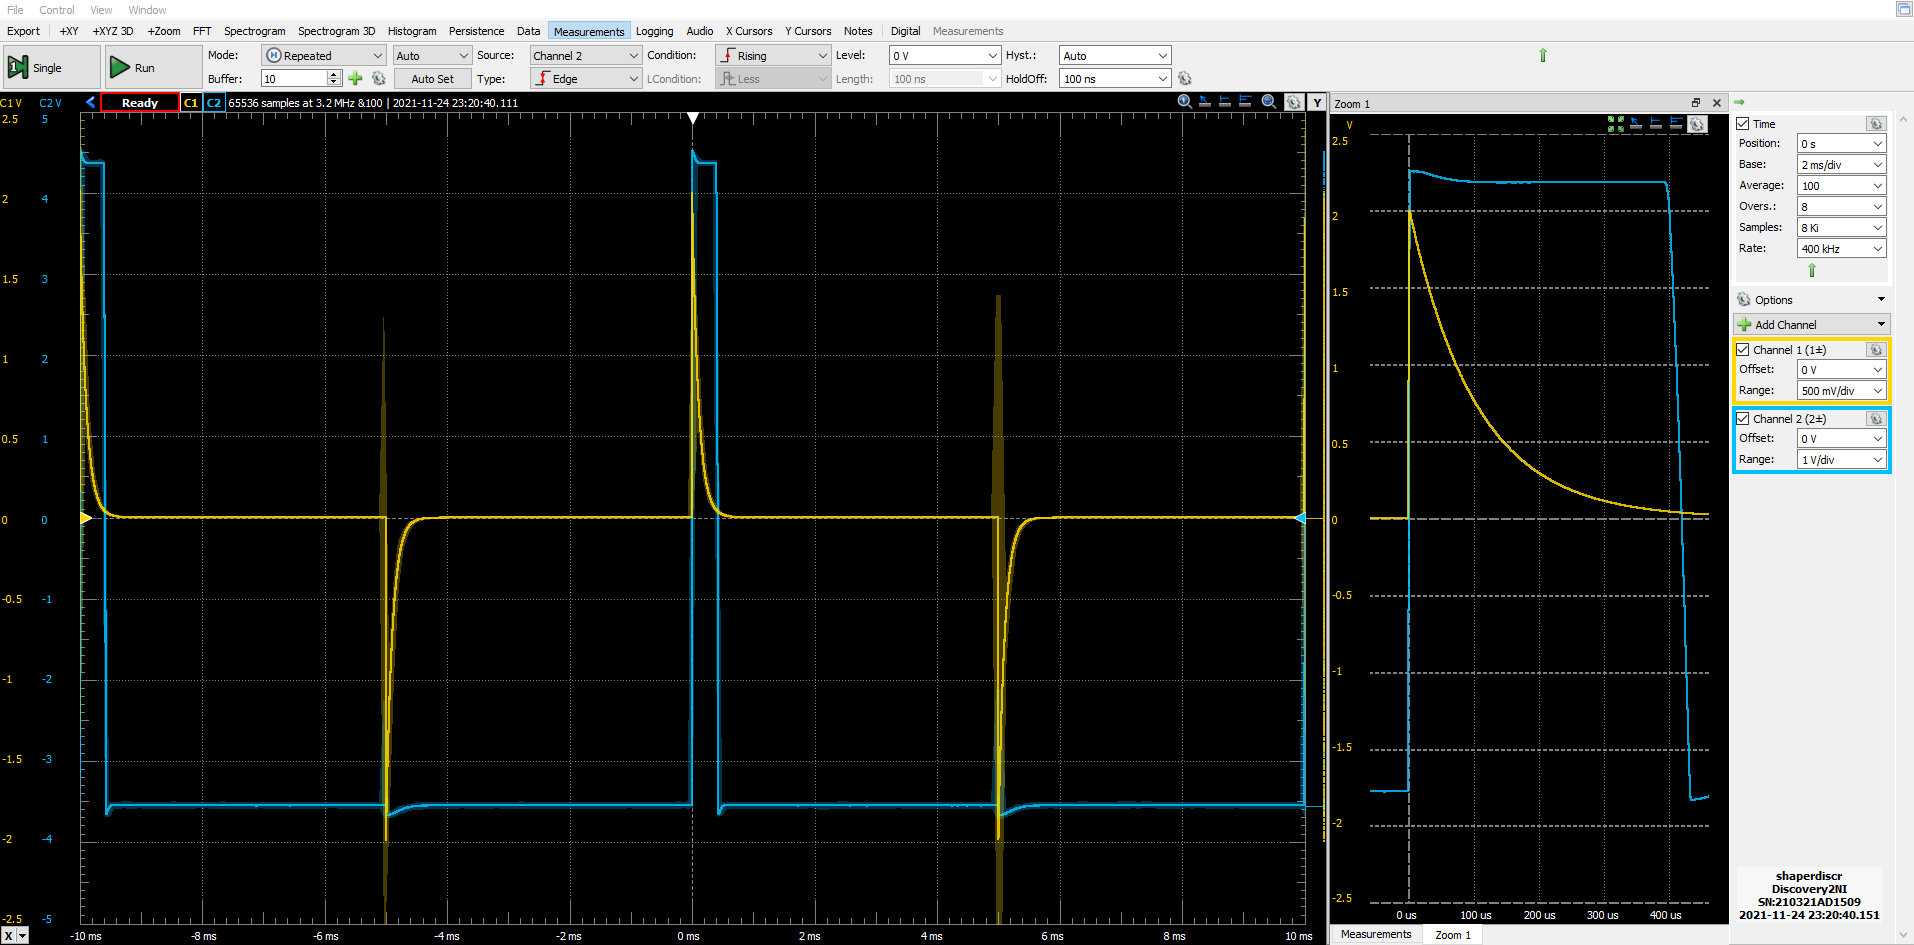
\includegraphics[scale=0.335]{shaper_discrzoom}
\caption{Acquisizione del segnale in uscita dal circuito discriminatore con
un'onda quadra in ingresso $V_s = \SI{1}{\V}$, $f = \SI{100}{\Hz}$
\label{fig: shaperdiscr}}
\end{figure}

\begin{figure}[htbp]
\centering
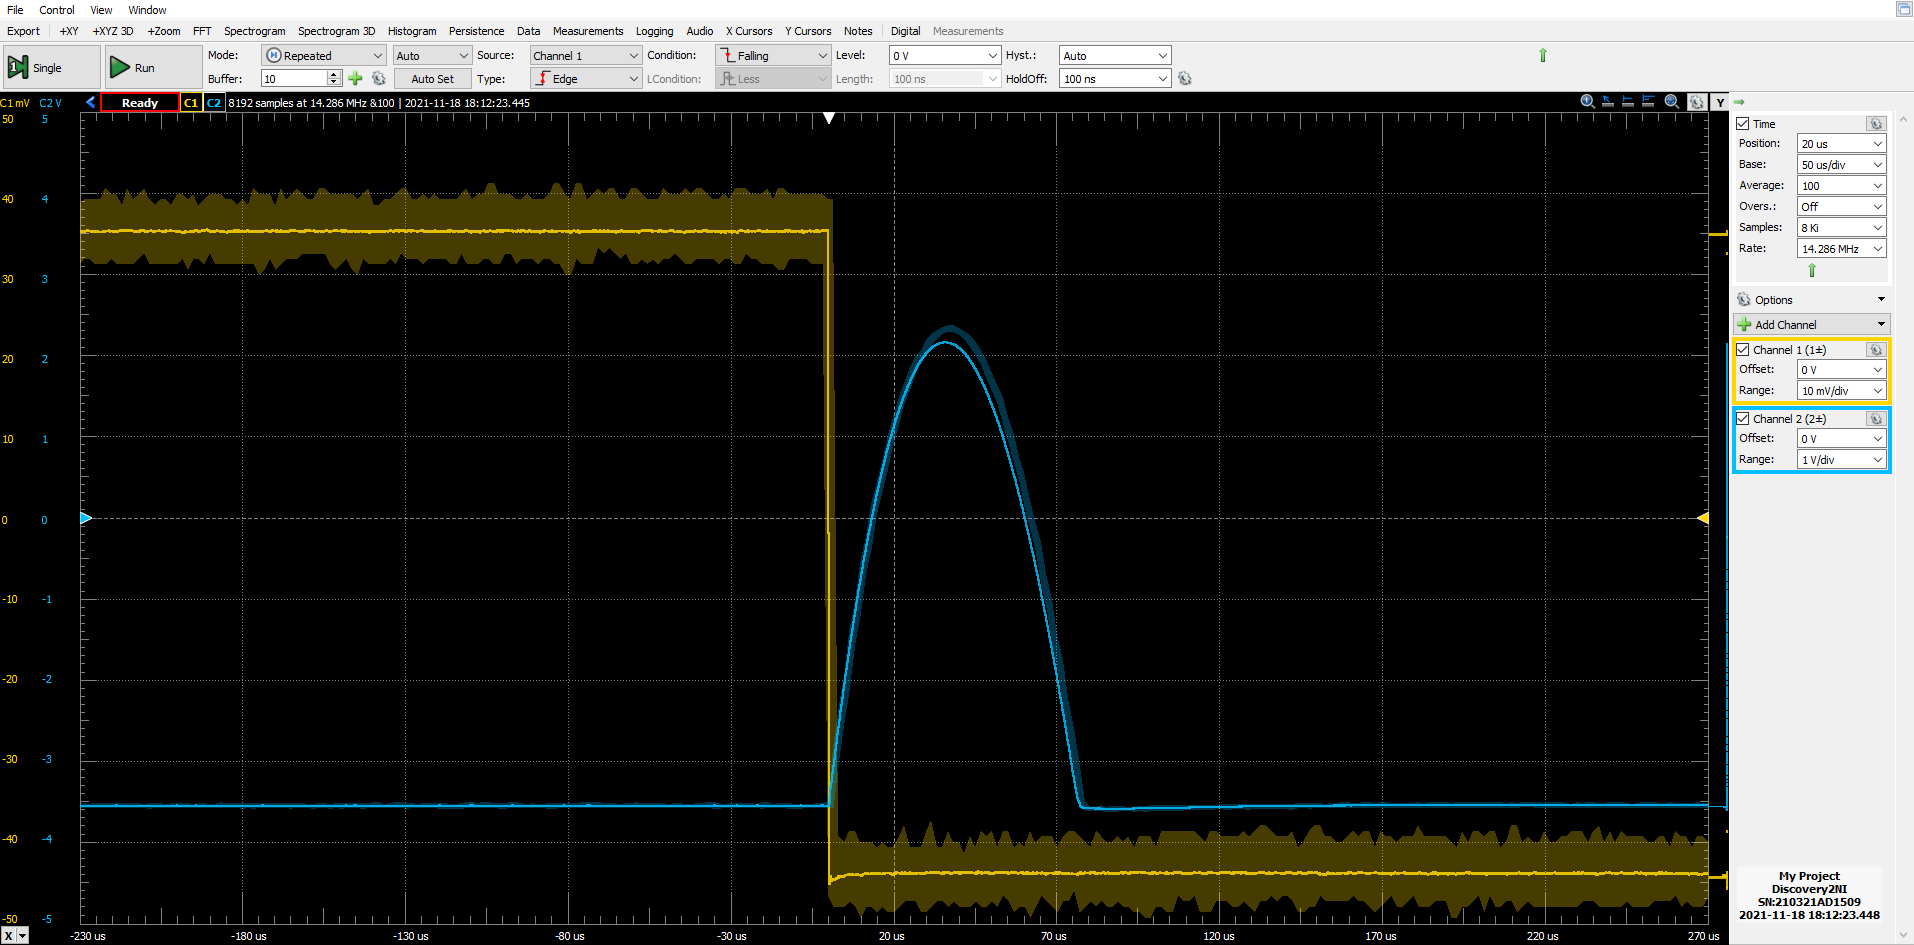
\includegraphics[scale=0.335]{discr_sat}
\caption{Acquisizione del segnale in uscita dal circuito discriminatore con
un'onda quadra in ingresso $V_s = \SI{30}{m\V}$, $f = \SI{100}{\Hz}$
\label{fig: discr_sat}}
\end{figure}
al di sotto dei $\SI{50}{m\V}$ invece il segnale in uscita inizia a deformarsi,
assumendo la forma di una parabola rovesciata che si sposta verso il basso
più diminuiamo l'ampiezza in ingresso

Il fronte di salita all'uscita del discriminatore è sicuramente limitato dallo
slew rate finito dell'amplificatore
\[
t_{oh} = V\ped{disc}^{pp}/SR = 7.9 / 13 = 2 \; \si{\micro\s}
\]
mentre il fronte di discesa è meno ripido perché corrisponde alla transizione
del discriminatore sulla discesa esponenziale di $V\ped{sh}$, che ha una derivata
piccola in prossimità della soglia. Questo infatti lascia presumere che esista
un intervallo temporale durante il quale l'uscita di $V\ped{discr}$ è in zona
lineare.

Infatti si è trovato, per ampiezza dell'onda quadra prossima alla soglia
\begin{figure}[htbp]
\centering
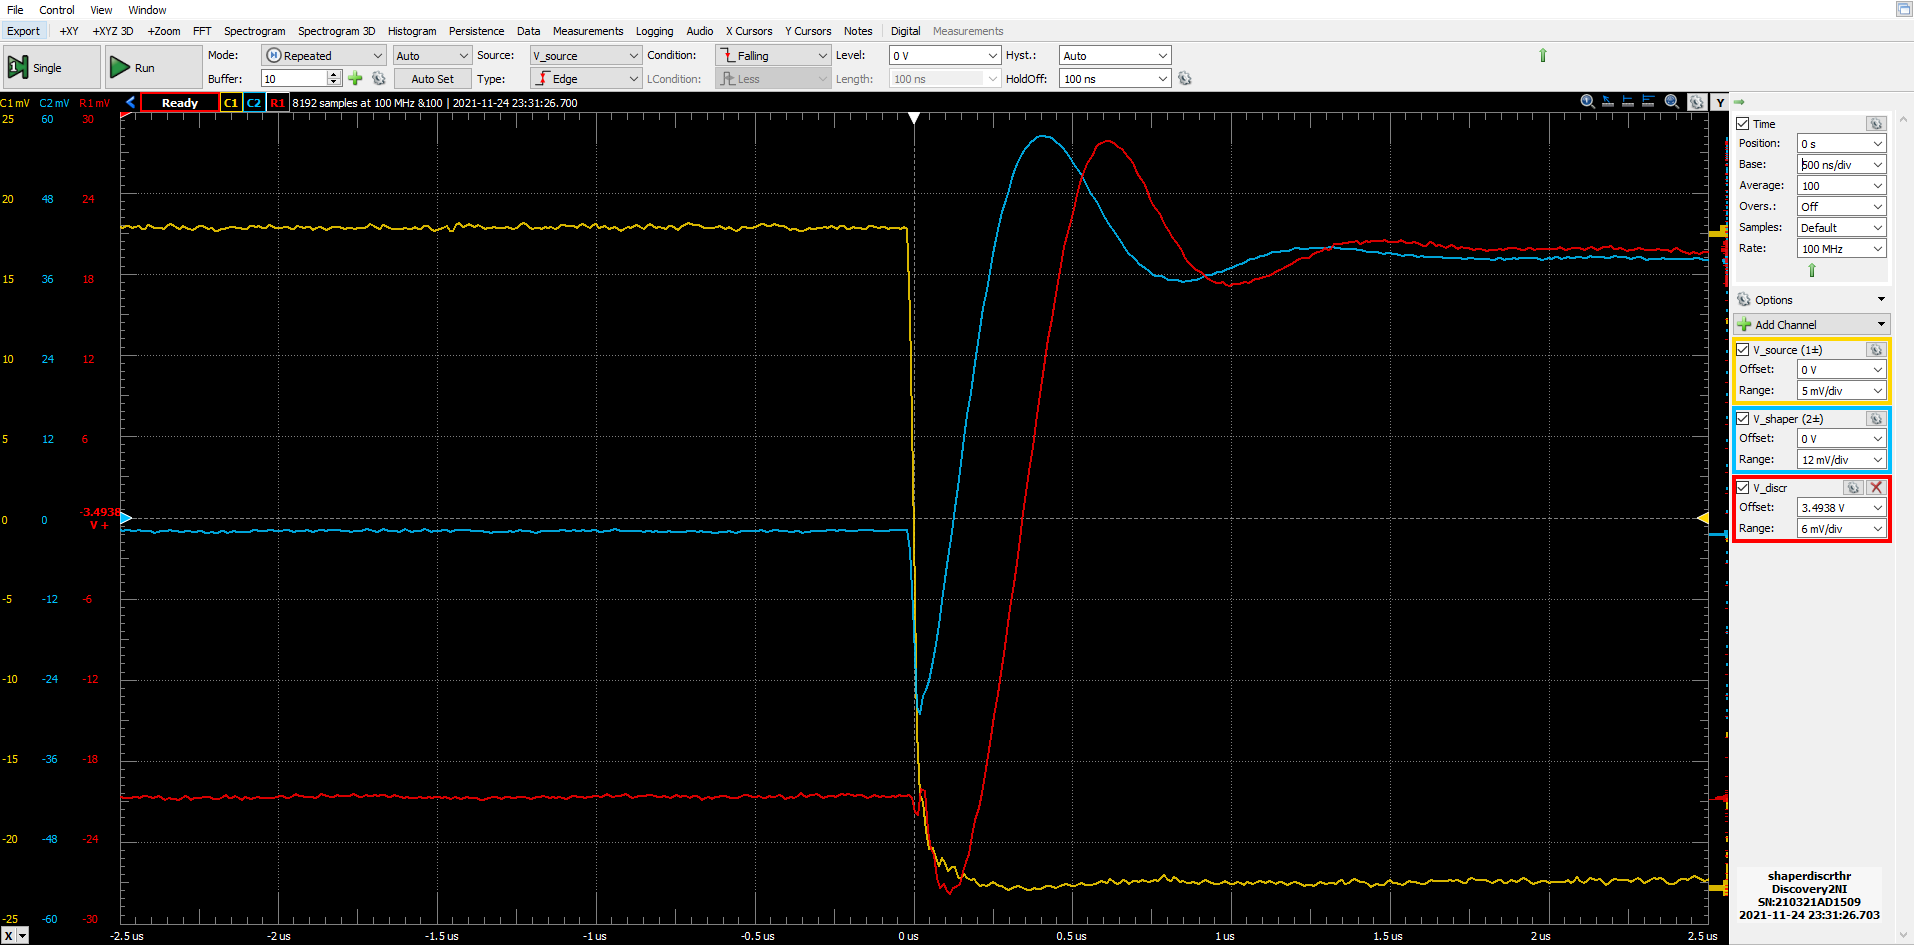
\includegraphics[scale=0.335]{shdiscthr}
\caption{Acquisizione del segnale in uscita dal circuito discriminatore con
un'onda quadra in ingresso $V_s = \SI{20}{m\V}$, $f = \SI{100}{\Hz}$
\label{fig: discrthr}}
\end{figure}
che è proprio il transiente dello shaper visto in \ref{fig: shzoom} amplificato
dal secondo OpAmp in regime lineare.

questo comportamento si osserva fino a circa $\SI{20}{m\V}$, quando il segnale
in uscita dal comparatore non è più apprezzabilmente diverso dalla tensione di
saturazione del trigger.

\subsection{Minima ampiezza di carica per cui si attiva il comparatore}
Per ottenere una misura di ampiezza minima di carica per cui si registra un
segnale che raggiunga la soglia $V_{OH}$ in uscita dal discriminatore abbiamo
variato l'ampiezza del segnale in ingresso $V_s$ dal generatore di forme
d'onda, dunque abbiamo misurato con i cursori l'ampiezza critica trovata per
i due circuiti studiati:
\begin{align*}
V\ped{min} &= 40.5 \pm 0.3 \; \si{m\V} \\ 
V\ped{min} &=  \pm  \; \si{m\V}
\end{align*}
che corrisponde ad una quantità di carica minima per l'amplificatore di
$Q\ped{min} = C_T \cdot 2V\ped{min} = 80 \pm  3 \; \si{\pico\coulomb}$.

\subsection{Confronto con i valori attesi}
Abbiamo eseguito un fit con legge logaritmica per l'andamento delle misure
del Time-over-Threshold al variare dell'ampiezza di carica in ingresso
$Q\ped{in}$, di cui riportiamo i risultati
\begin{figure}[htbp]
    \centering
	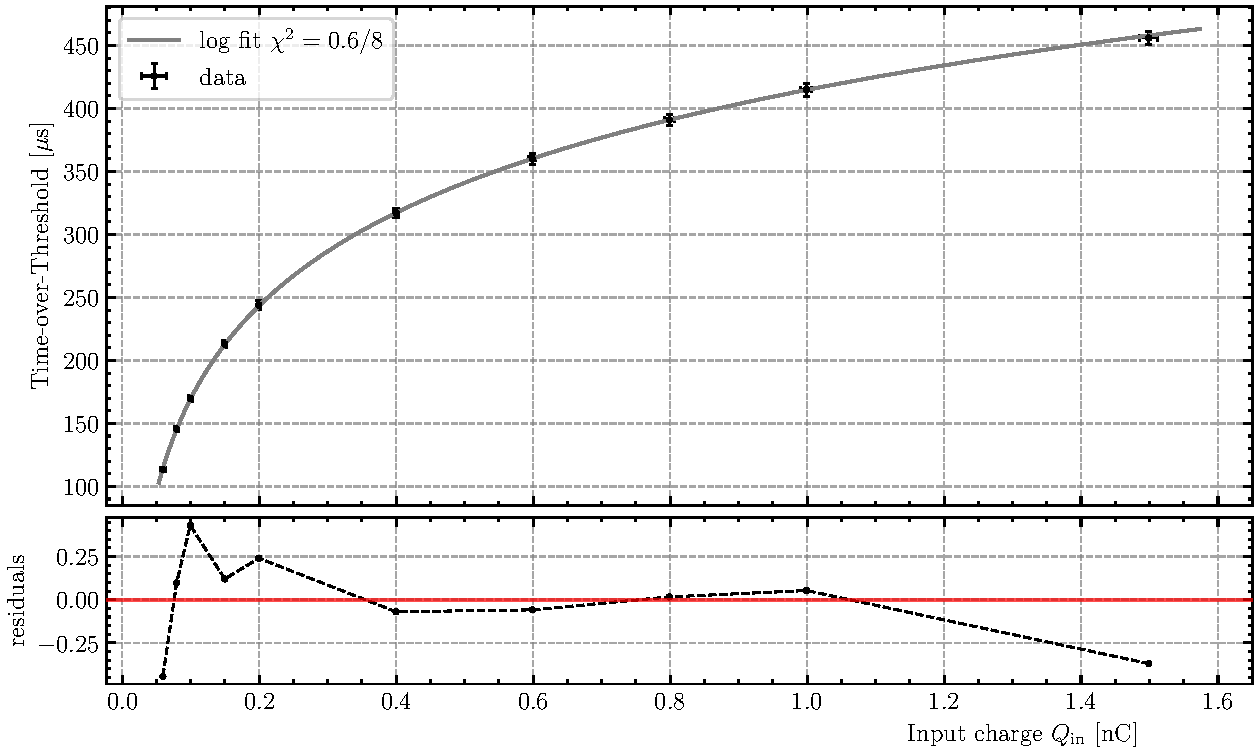
\includegraphics[scale=0.7]{logfit}
    \caption{Fit logaritmico del $ToT$ in funzione dell'ampiezza di carica in
    ingresso $Q\ped{in}$ \label{fig: logfit}}
\end{figure}
\begin{align*}
V\ped{thr} &= 40.7 \pm 0.2 \; \si{m\V}
&\tau = 106.51 \pm 0.3 \; \si{\micro\s} \\
\chi^2/\mathrm{ndof} &= 0.6/8 &\mathrm{cov_{norm}} = 0.82
\end{align*}

Ritroviamo che il valore del tempo di smorzamento $\tau$ è compatibile con il
valore atteso dai componenti del circuito.
e che la tensione di soglia trovata dal fit è compatibile con il valore
in corrispondenza della minima ampiezza di carica.
%=======================
\section{Trigger di Schmitt}

\begin{figure}[htbp]
    \centering
	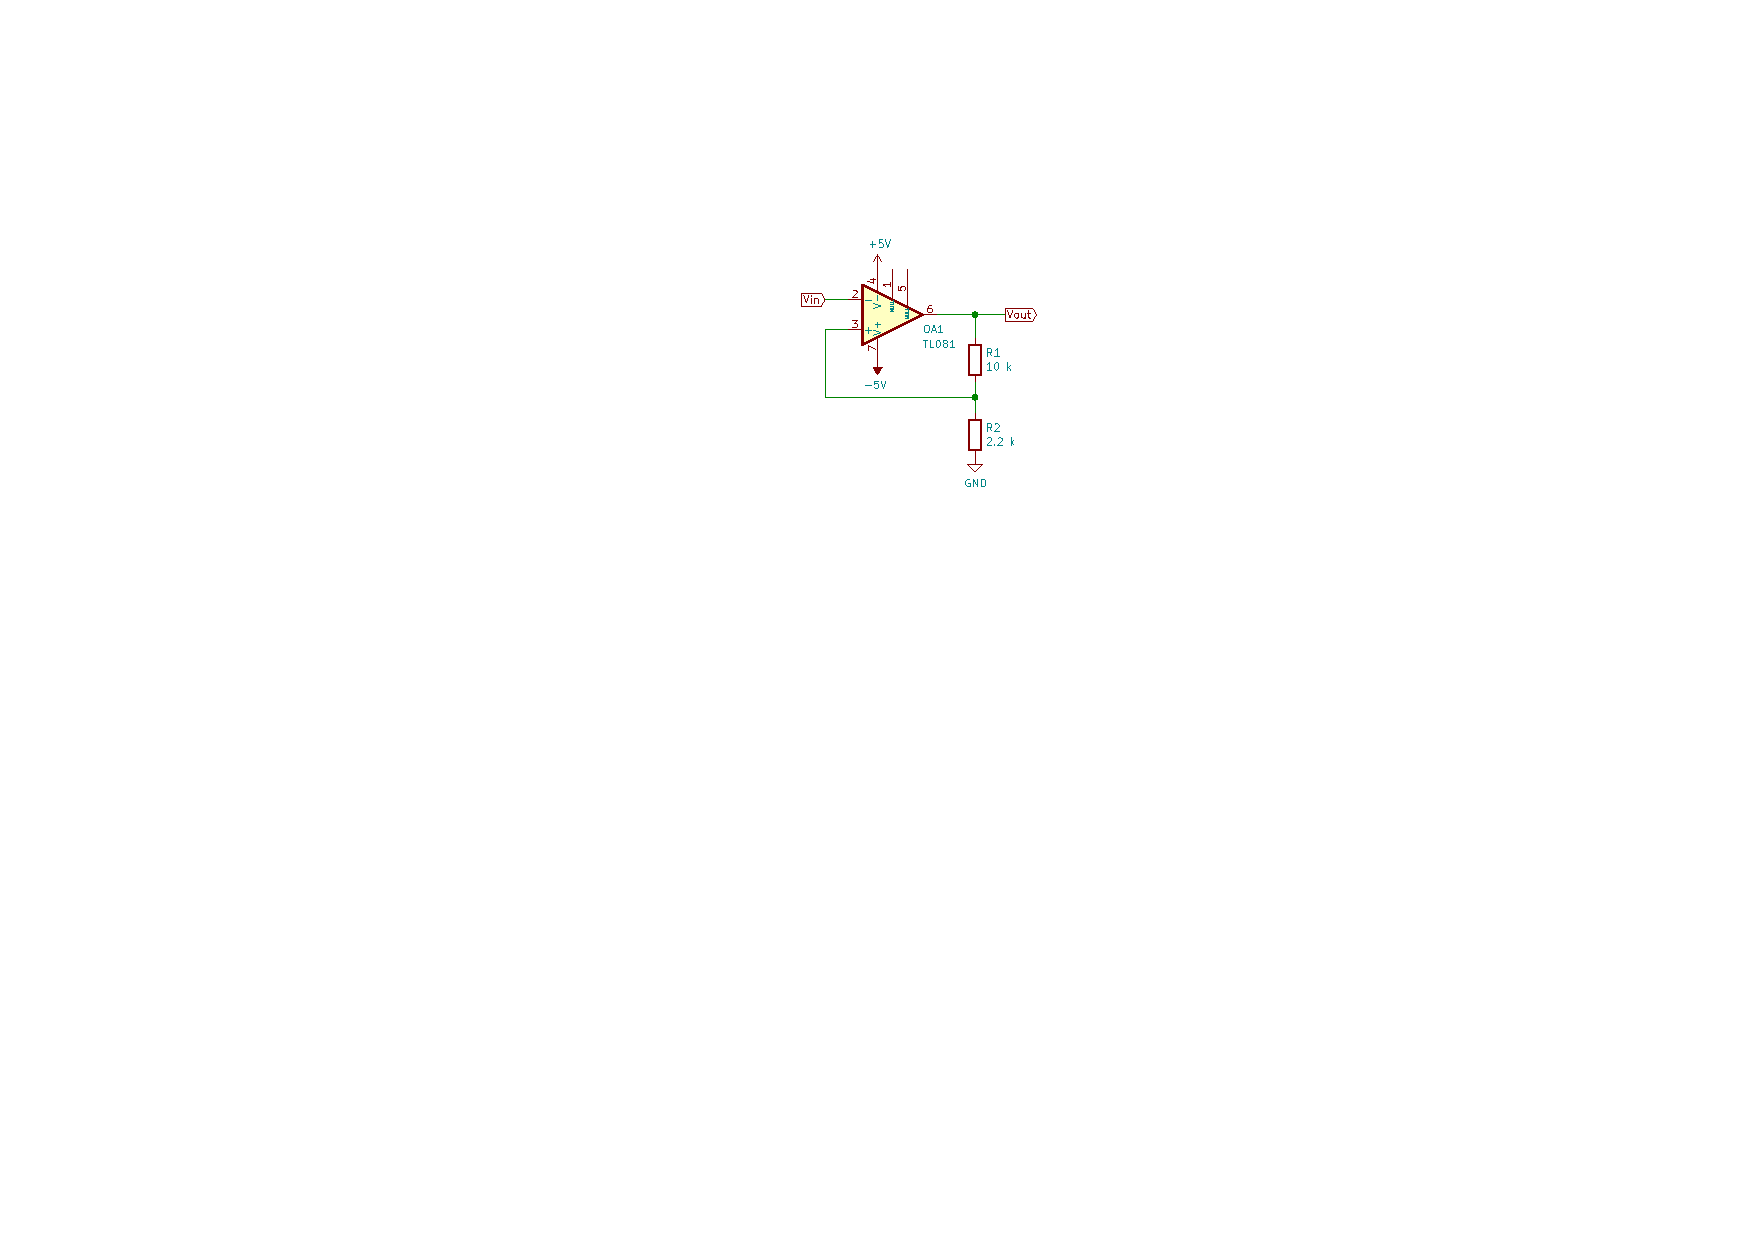
\includegraphics[scale=1.5]{trgSchmitt}
    \caption{Schema circuitale del trigger di Schmitt costruito.
    \label{fig: trgschmittschm}}
\end{figure}

\subsection{Risposta ad un'onda sinusoidale}

\begin{figure}[htbp]
\centering
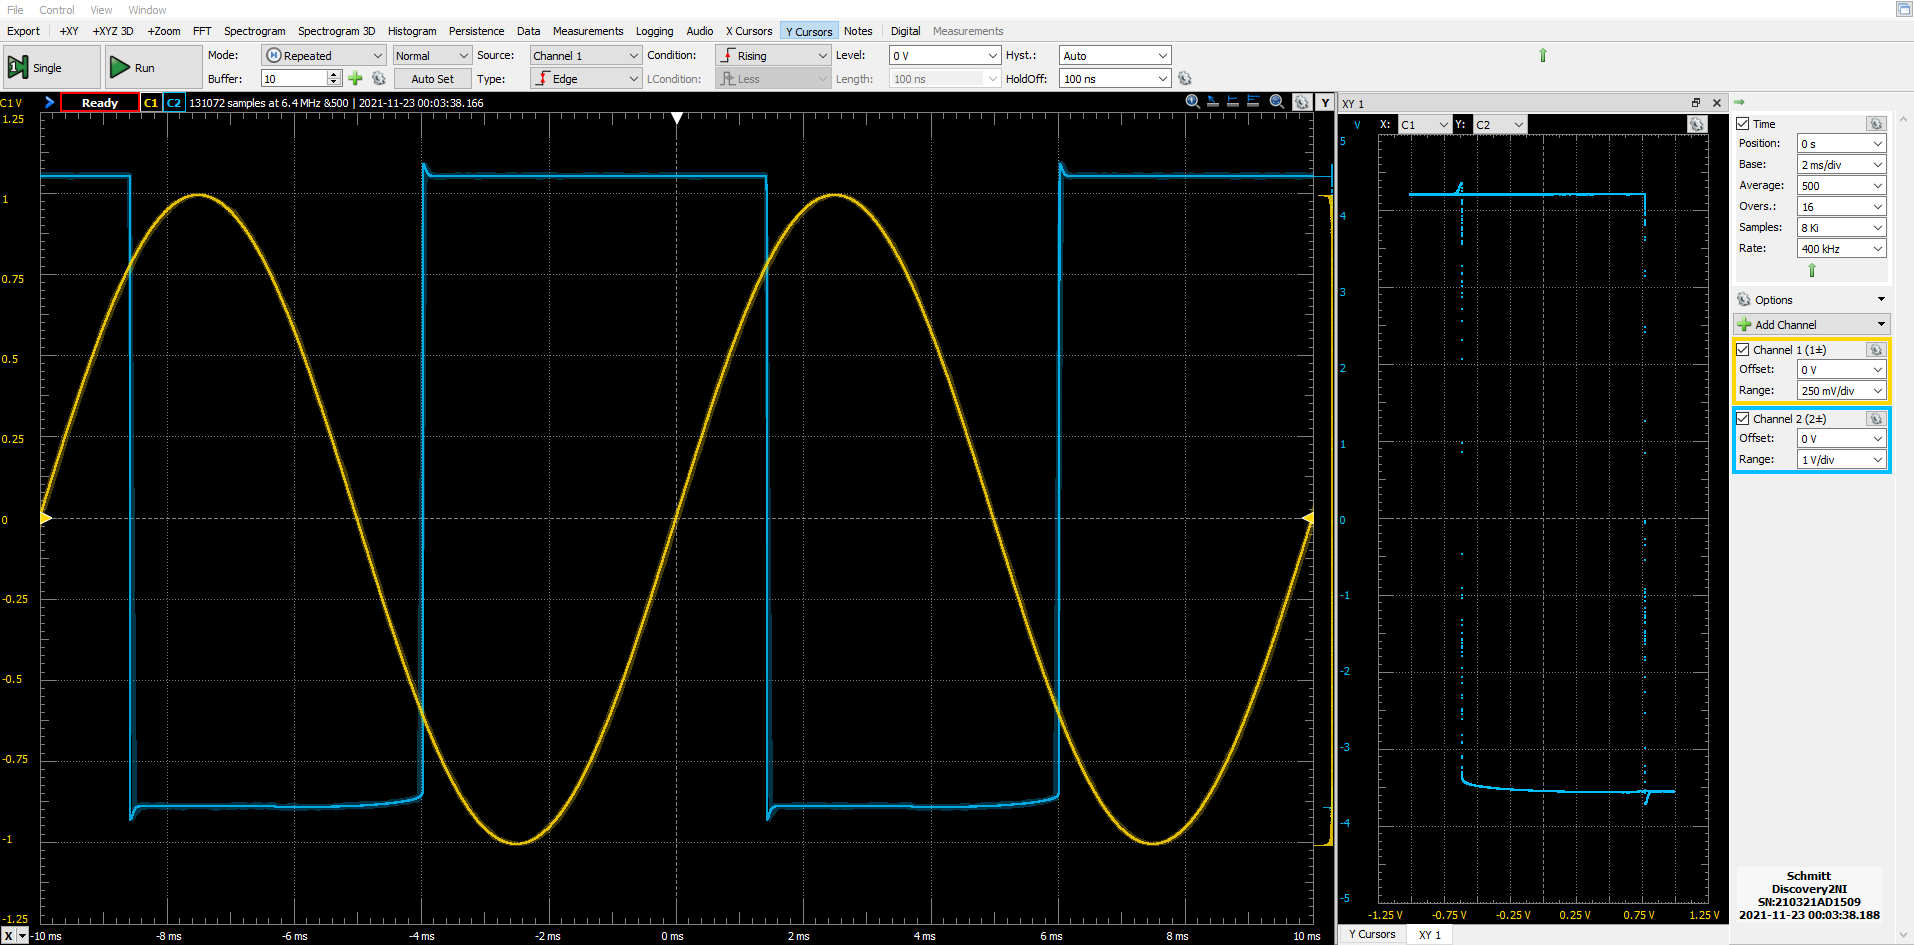
\includegraphics[scale=0.335]{schmitt}
\caption{risposta ad un segnale sinusoidale di ampiezza 1 V e frequenza 100 Hz del trigger di schmitt}
\end{figure}

\begin{figure}[htbp]
\centering
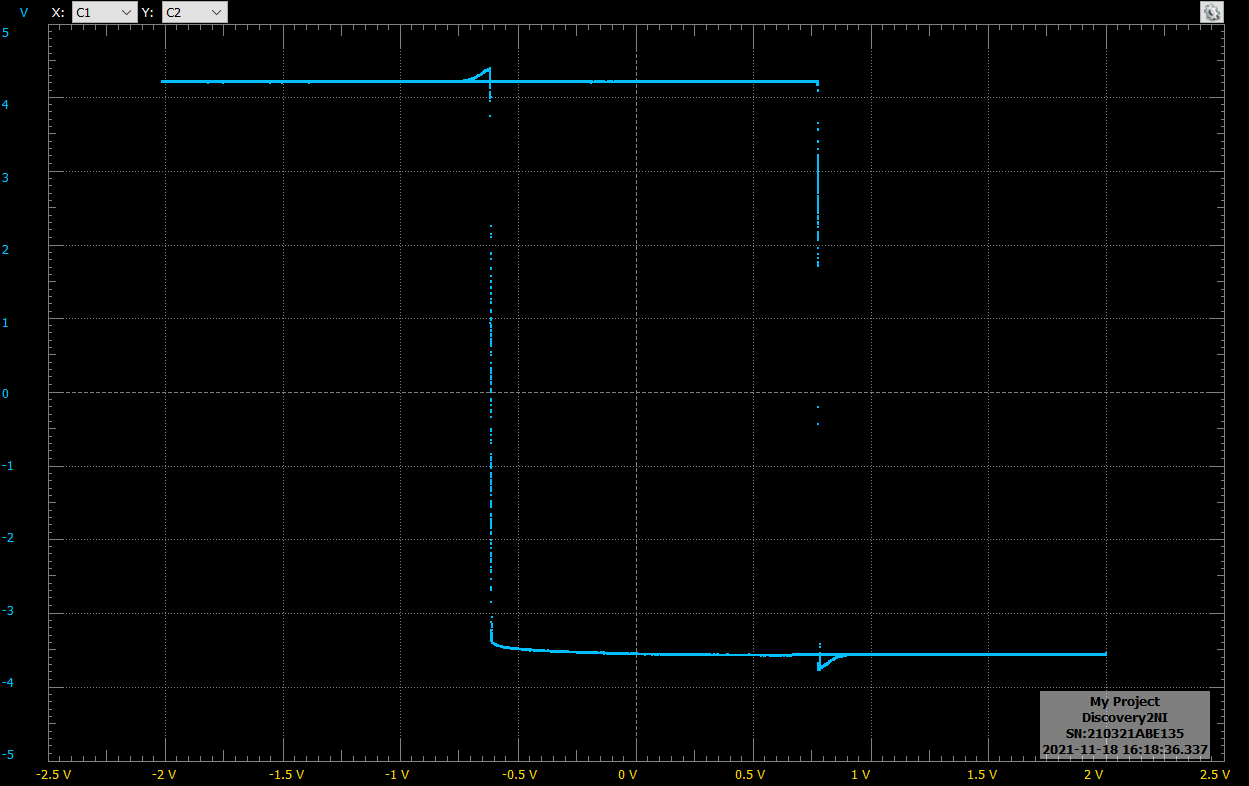
\includegraphics[scale=0.4]{shmitt_isteresi}
\caption{risposta ad un segnale sinusoidale di ampiezza 2 V e frequenza 100 Hz del trigger di schmitt, visto nel piano XY in cui il segnale in ingresso è sulle x e il segnale in uscita sulle y}
\end{figure}


\subsection{Saturazione dell'OpAmp}
Per il primo circuito 
\begin{align*}
V_{OH} = 4.28 \pm 0.04 \; \si{\V} \\
V_{OL} = -3.66 \pm 0.03 \; \si{\V}
\end{align*}
Mentre per il secondo
\[
V_{OH} = 4.21 \pm 0.04 \; \si{\V}
\]
\[
V_{OL} = -3.53 \pm 0.03 \; \si{\V}
\]
\subsection{Tensioni di soglia e funzionamento del trigger}
Abbiamo inviato in ingresso all'amplificatore un'onda sinusoidale di ampiezza
$1999 \pm 15 \; \si{m\V}$ e frequenza $1000 \pm 16 \; \si{\Hz}$.
Dalle intersezioni tra i due canali abbiamo misurato le transizioni basso-alto
(OH) e alto-basso (OL)

\begin{align*}
V_{TH} = -617 \pm 5 \; \si{m\V} \\
V_{TL} = 775 \pm 6 \; \si{m\V}
\end{align*}
Per il secondo circuito invece è stata fatta una media pesata sui punti sulle 2 linee verticali che si formano nel grafico XY (ovviamente una per ogni linea).
\[
V_{TH} = 611.6 \pm 0.5 \; \si{m\V}
\]
\[
V_{TL} = 780.4 \pm 0.5 \; \si{m\V}
\]

Supponiamo che l'OpAmp funzioni come discriminatore, cioè che la differenza tra $v_+ $ e $v_- $ sia tale da farlo lavorare sempre in regime non lineare. Allora vale
\[ V\ped{out} = V_{CC} \sgn(v_+ - v_-). \]
Inoltre, poiché $v_+ $ è collegato all'uscita del partitore, abbiamo
\[ v_+ = \frac{R}{R_1 + R_2} V \ped{out} = \beta V\ped{out} \]
e quindi
\[
V\ped{out} = V_{CC} \sgn(\beta V\ped{out} - V_s)
.\]
Da questa si conclude che il valore di $V\ped{out} $ sarà ``alto''
(cioè pari a $ V_{CC} $ nel semipiano $V\ped{out} > \frac{V_s}{\beta}$ e
``basso'' nel semipiano $ V \ped{out} < \frac{V_s}{\beta}$. La transizione
avviene pertanto quando si ha
\[
V_s = \pm V \ped{sat} \qquad\text{con}\qquad V \ped{sat} = \beta V_{CC} = \frac{R_2}{R_1 + R_2} V_{CC}
\]

Che corrisponde ad un valore di soglia $V\ped{sat} = 0.90 \pm 0.03 \; \si{\V}$

Il feedback positivo regola il funzionamento del trigger tramite il controllo del segnale in ingresso. Se la tensione $V_s$ è minore di $V_{TH}$ il segnale in uscita rimane sul livello alto. Aumentando l’ampiezza del segnale in ingresso fino a superare il valore di soglia $V_{TH}$ il circuito salta bruscamente dal segnale a livello alto a quello a livello basso. Segue un ragionamento analogo per il restante periodo dell’onda tenendo in considerazione $V_{TL}$, con l’ampiezza del segnale in ingresso che
diminuisce fino a $V_{OL}$


\subsection{Limiti fisici del circuito}
\[
F_{L} = 92.6 \pm 0.1 \; \si{k\Hz}
\]
\[
SR = 11.1 \pm 0.3 \; \si{\V/\micro\s}
\]
\begin{figure}[htbp]
\centering
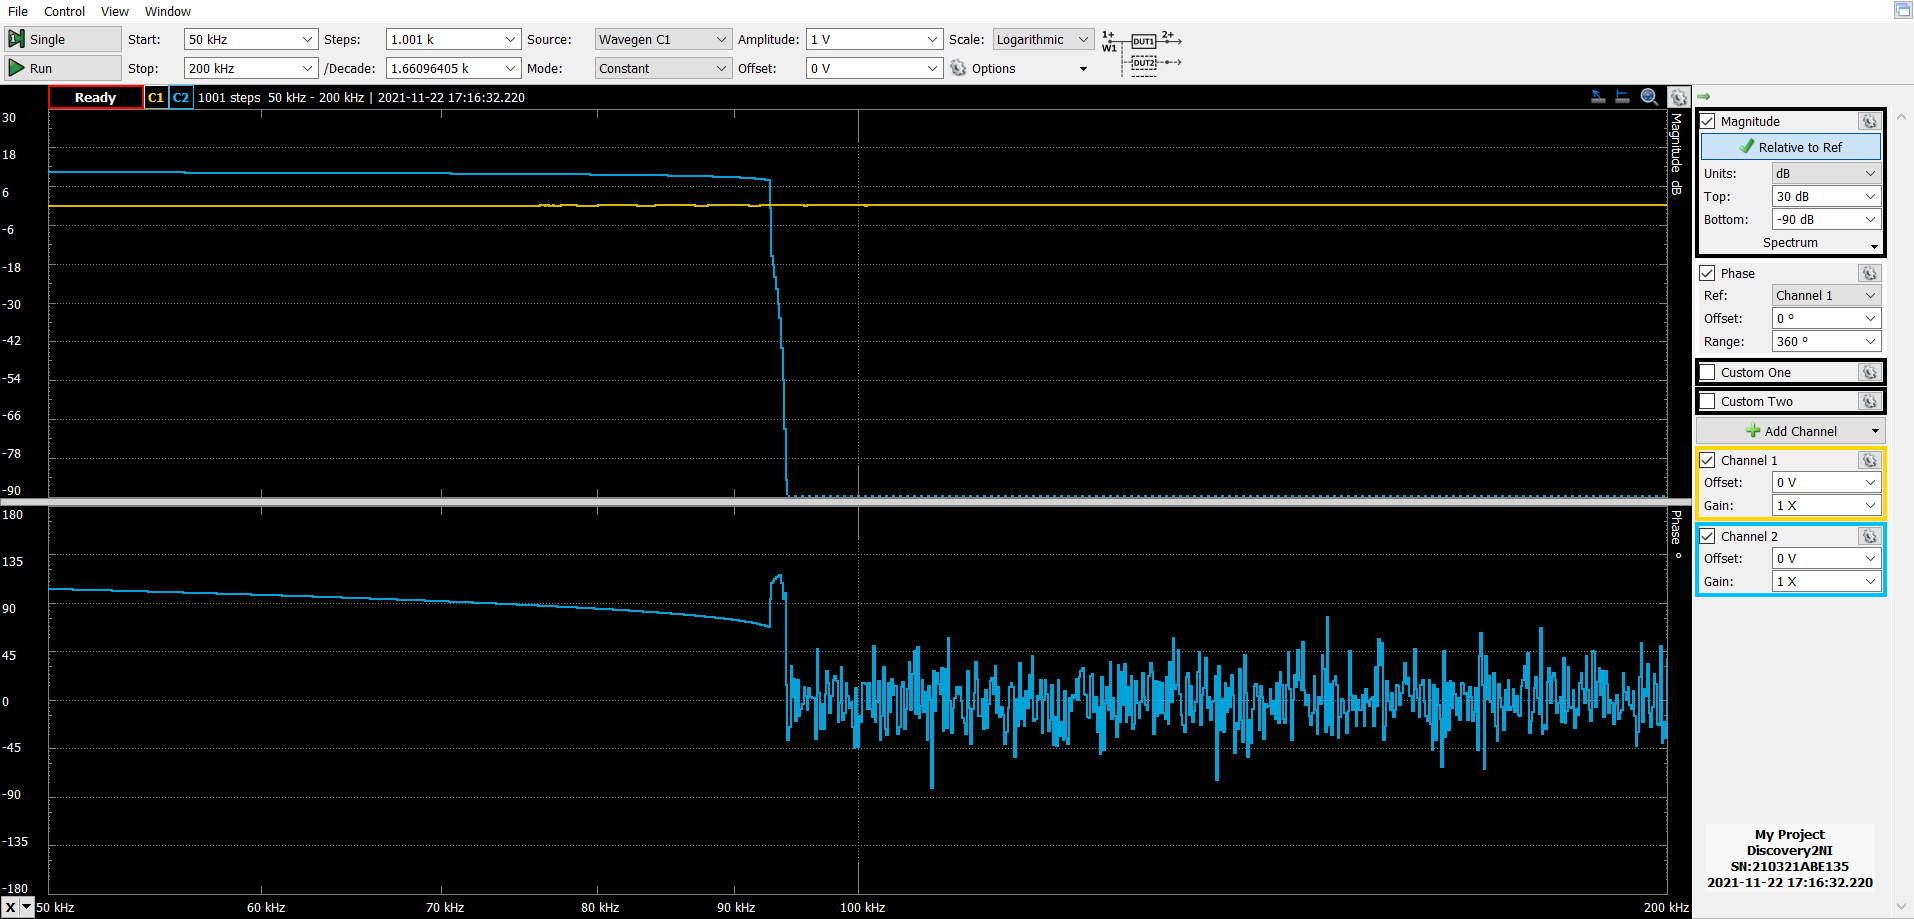
\includegraphics[scale=0.4]{schmitt_freq}
\caption{analisi in frequenza del trigger di schmitt, in particolare l'unico punto di interesse si trova a circa 90 kHz, punto in cui smette di funzionare}
\end{figure}

Si osserva che il circuito si comporta come discriminatore con isteresi per
frequenze sufficientemente basse. Per frequenze maggiori di
$\sim\SI{10}{\kilo\hertz}$ la pendenza della transizione del segnale in
uscita da ``alto'' a ``basso'' e viceversa comincia ad essere limitata dallo
slew rate dell'OpAmp.

Il regime in cui l'OpAmp si comporta da discriminatore con isteresi è quello
in cui il tempo minimo di salita e discesa è molto minore del periodo del
segnale in ingresso (e in uscita)
\begin{equation}\label{eq:slewlimit}
T \gg 2 t \ped{min} \qquad t \ped{min} = \frac{V\ped{out}}{\mathrm{SR}} \approx \SI{0.5}{\micro\second} \implies f \ll \SI{1}{M\hertz}.
  \end{equation}

Variando l'ampiezza del segnale in igresso $V_s$ si osserva che l'ampiezza del
segnale in uscita rimane pressoché uguale fino a una soglia inferiore, al di
sotto della quale diventa costante. 
Infatti, affinché ciò non accada il circuito deve poter compiere il ciclo di
isteresi, e dunque l'ampiezza picco-picco del segnale in ingresso deve essere
maggiore della base del rettangolo di isteresi:
\[ V_s > 2 V \ped{sat} \eqqcolon V\ped{s, min}. \]

Sperimentalmente, si misura come ampiezza in ingresso minima

%=======================
\section{Multivibratore astabile}

\begin{figure}[htbp]
    \centering
	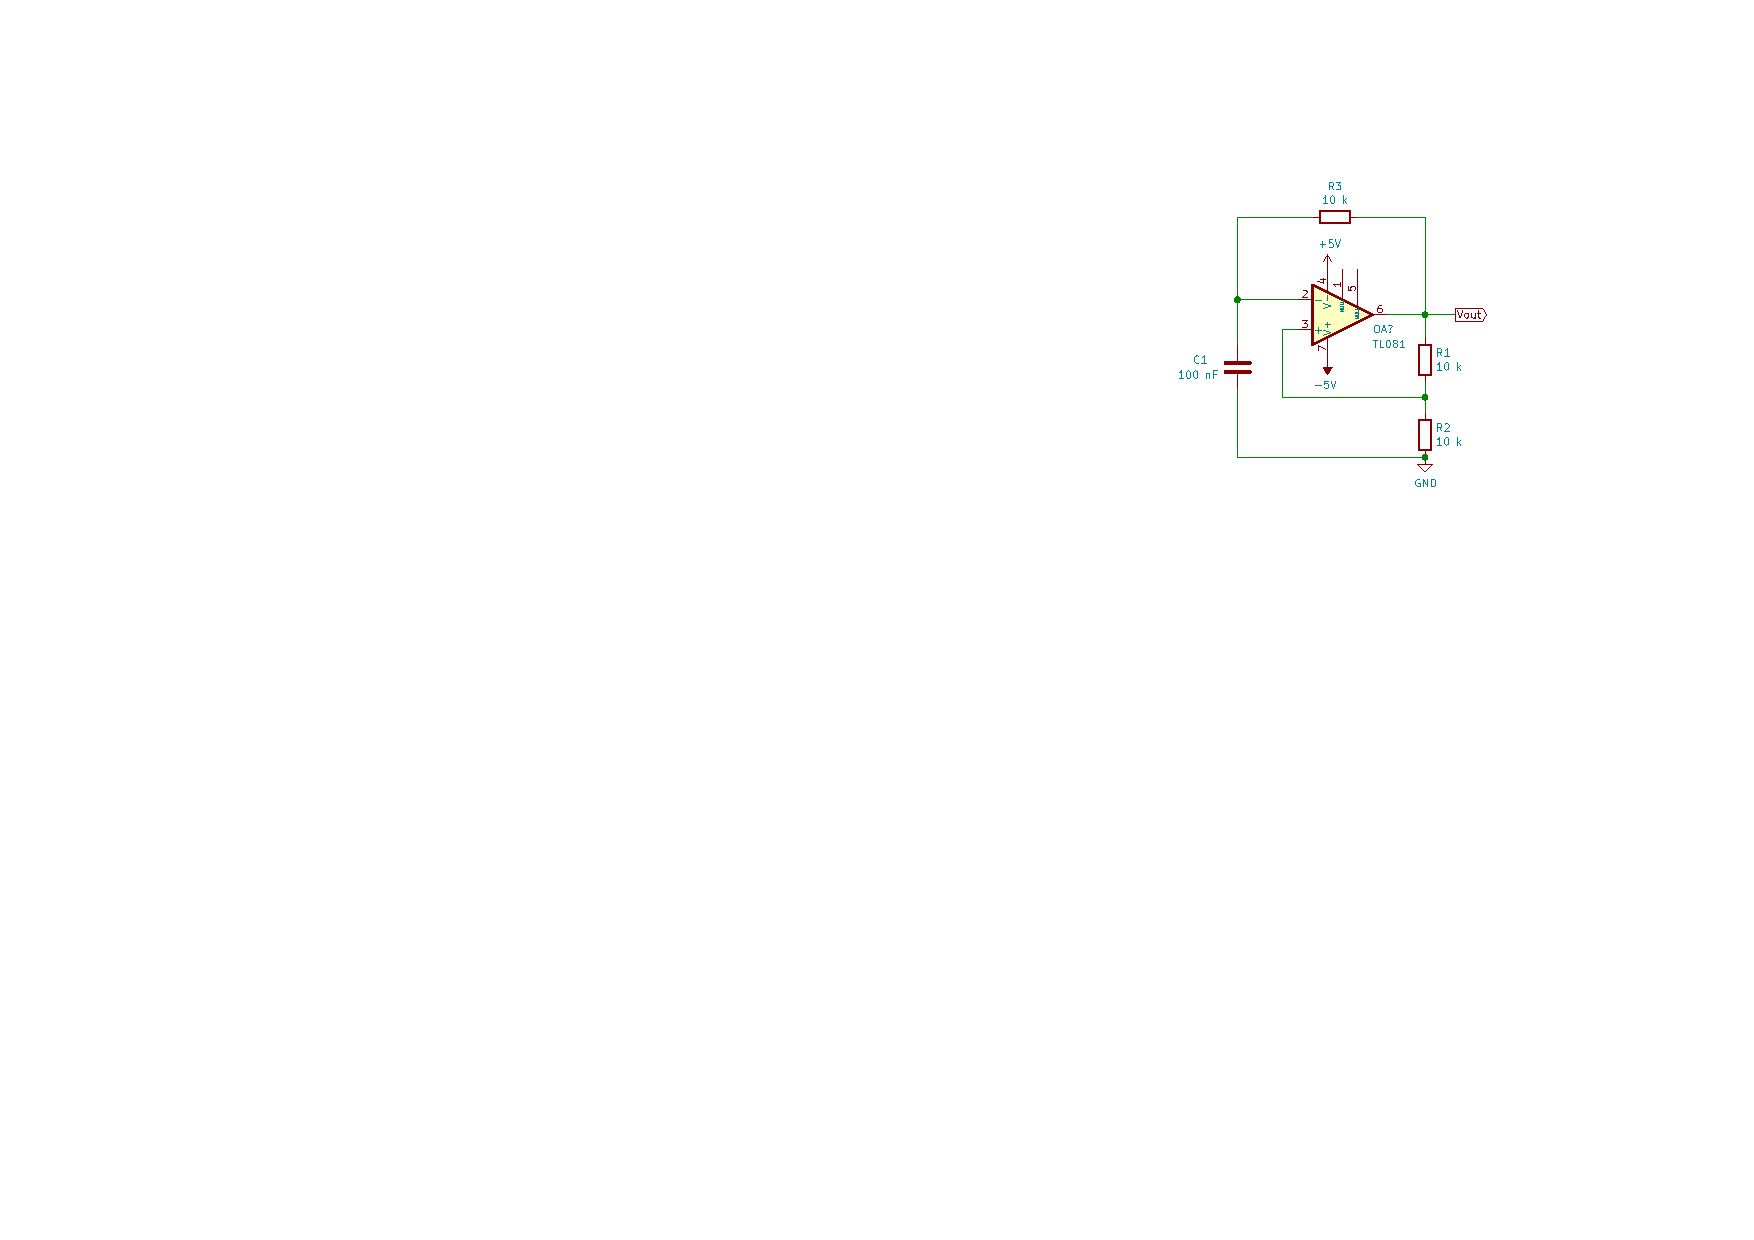
\includegraphics[scale=1.5]{astable}
    \caption{Schema circuitale del multivibratore astabile costruito.
    \label{fig: astableschm}}
\end{figure}

\subsection{Funzionamento del circuito}
Il circuito in figura \ref{fig: astableschm} funziona come un trigger di
Schmitt collegato in input ad un filtro passa-basso RC. Il condensatore $C_1$ si
carica fino a raggiungere il livello della tensione dell’ingresso non
invertente, a questo punto l’OpAmp scatta, la tensione nell’ingresso non invertente
scende e il condensatore comincia a scaricarsi fino a quando il livello della
tensione ai capi del condensatore non raggiunge quello presente all’ingresso
non invertente.
Il ciclo dunque si ripete generando un'onda quadra il cui periodo di
oscillazione è quindi il doppio del tempo caratteristico $\tau$ in
cui il condensatore è in grado di caricarsi/scaricarsi.
Dette
\begin{align*}
q &= \frac{R_1}{R_1 + R_2} \\
\tau &= R_3 C_1 = 101 \pm 4 \; \si{\micro\s}
\end{align*}
Abbiamo come valori attesi per i tempi caratteristici alto $t_H$ e basso
$t_L$ ed il periodo $T$ dell'onda quadra generata dal multivibratore:
\begin{align}
t_H &= \tau \ln\left(\frac{1 - q\frac{V_{OL}}{V_{OH}}}{1-q}\right) \\
t_L &= \tau \ln\left(\frac{1 - q\frac{V_{OH}}{V_{OL}}}{1-q}\right) \\
T &= 2 R_3 C_1 \ln\left(\frac{1 + q}{1 - q}\right) = t_H + t_L
\end{align}

\setcounter{subsection}{2}
\subsection{Studio dei segnali in ingresso e uscita}

\begin{figure}[htbp]
\centering
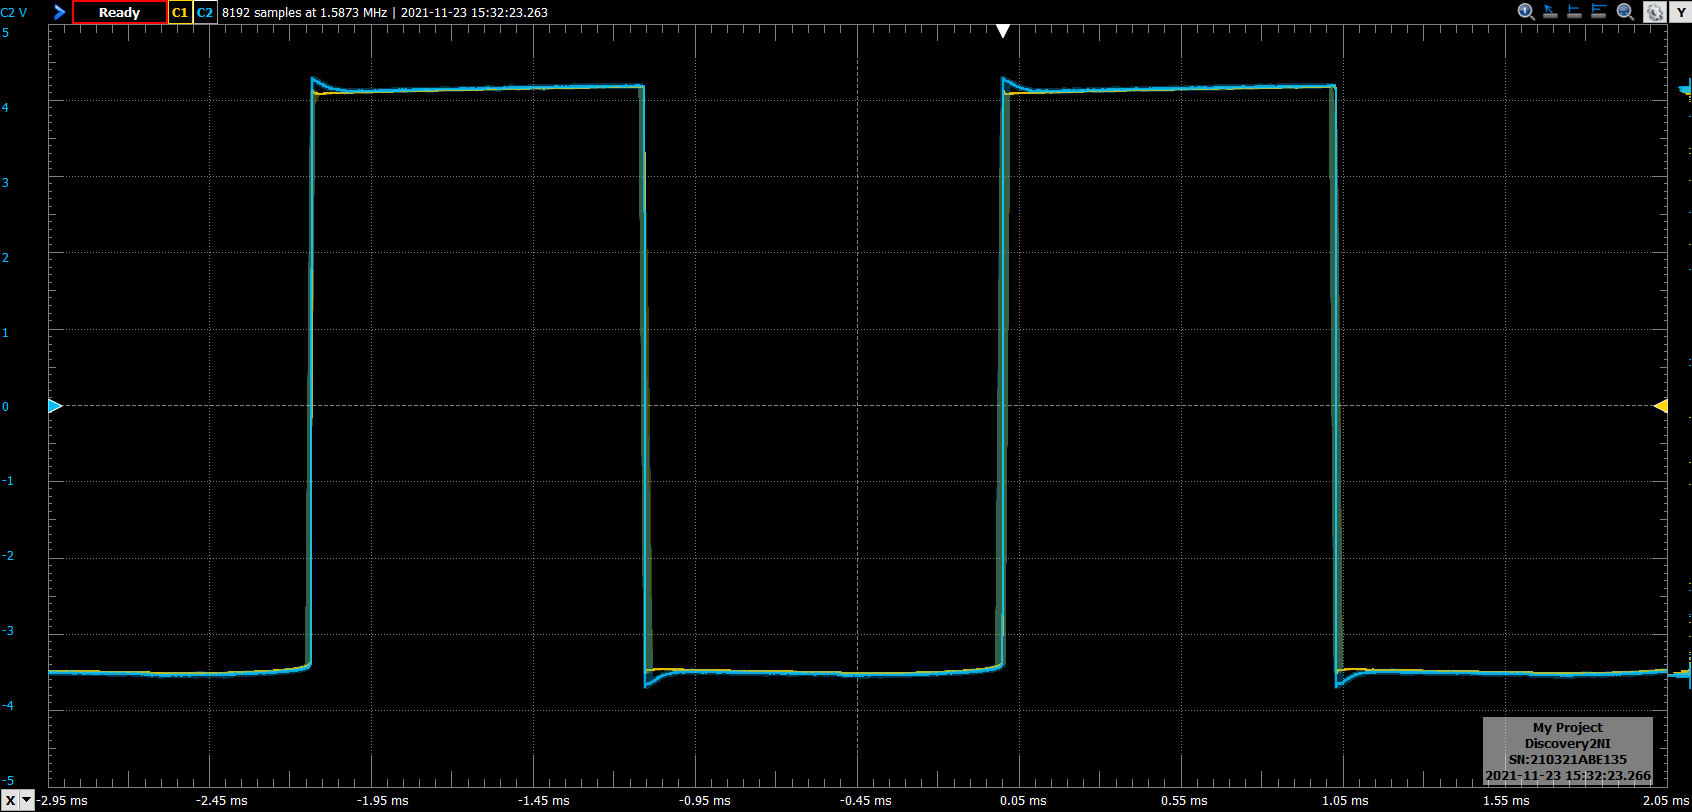
\includegraphics[scale=0.4]{V+Vout}
\caption{Grafico segnale in $V_+$ e segnale in $V_{out}$}
\end{figure}

\begin{figure}[htbp]
\centering
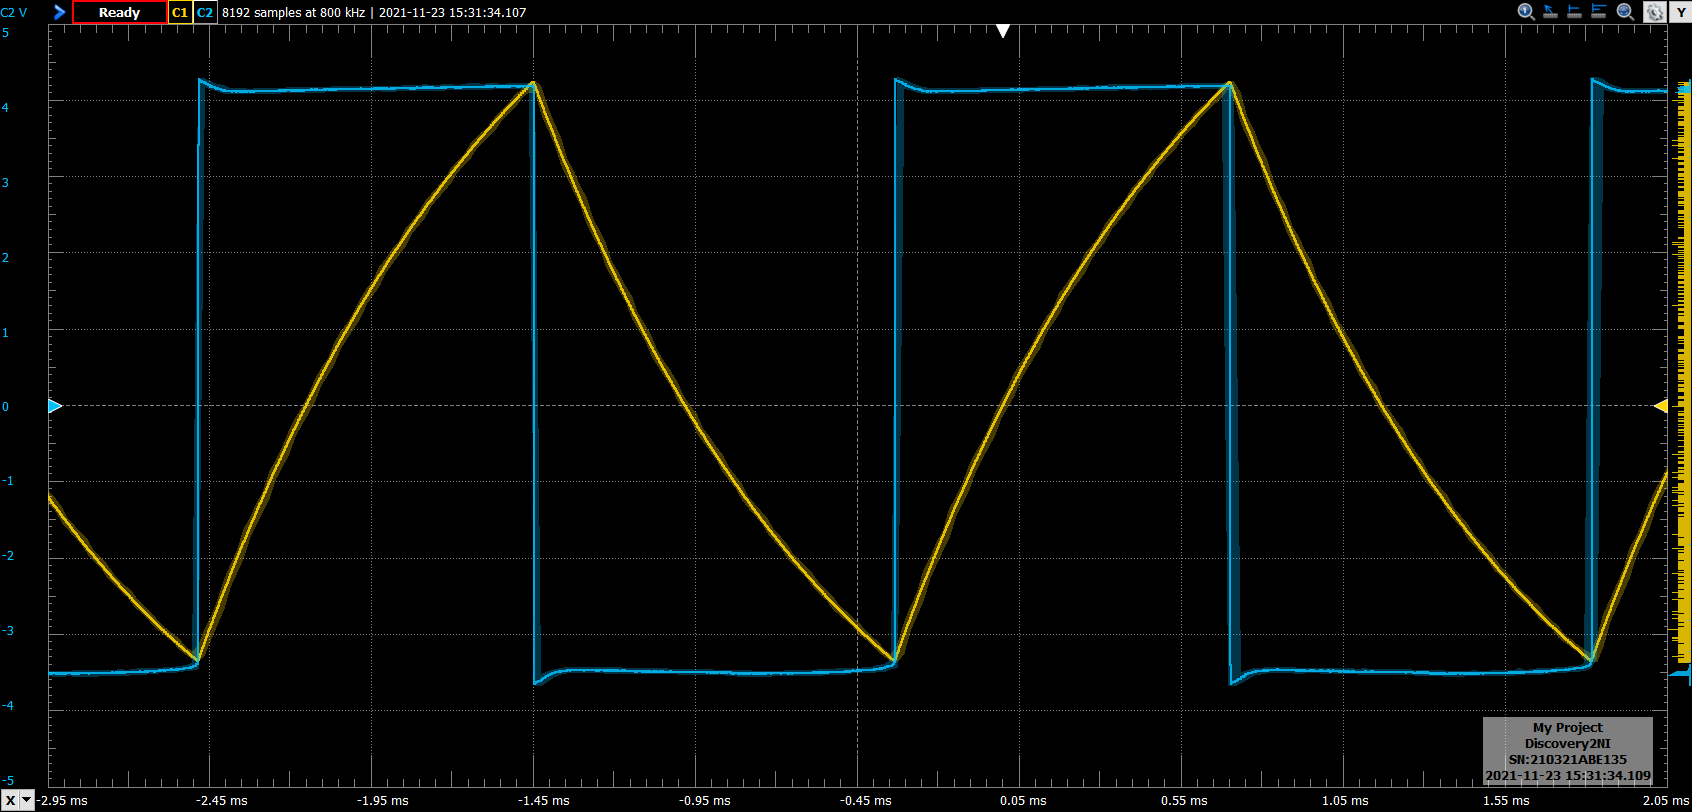
\includegraphics[scale=0.4]{V-Vout}
\caption{Grafico segnale in $V_-$ e segnale in $V_{out}$}
\end{figure}

Osservando il segnale in uscita Vout ci si aspetta di osservare un’onda quadra
di ampiezza picco-picco $\approx \SI{8}{\V}$ e periodo $2.15 \pm 0.03 \; \si{m\s}$ e
duty cycle $50 \%$.
Osservando $V_+$ ci si aspetta un segnale identico a $V\ped{out}$, ma ridotto di
un fattore $\beta \approx 0.5$.
Osservando $V_-$, infine, ci si aspetta di vedere un segnale ``a pinna di
squalo'', caratteristico del processo di carica/scarica di un condensatore,
con la stessa ampiezza picco-picco di $V_+$.

\subsection{Misure di periodo e duty cycle}

\[
DC = 0.482 \pm 0.013
\]
\[
T = 2.15 \pm 0.02 \si{m\s}
\]
\[
T_{atteso} = 2.17 \pm 0.09 \si{m\s}
\]

\subsection{Limite massimo in frequenza del generatore}
Riducendo di metà il valore della resistenza $R_3$ o riducendo di metà il
valore della capacità $C_1$ notiamo un raddoppiamento della frequenza
del treno d'impulsi generato dovuto ad un dimezzamento del tempo
caratteristico di carica/scarica $\tau=R_3 C_1$.

Quando il valore del periodo diventa dell'ordine del $\si{\micro\s}$, il
tempo che lo slew rate impiega per fare un salto di circa $8$V, non
otteniamo più in uscita un'onda quadra perché l'OpAmp non riesce a passare
in tempo da uno stato all'altro.

%=======================
\section{Multivibratore monostabile}
\begin{figure}[htbp]
    \centering
	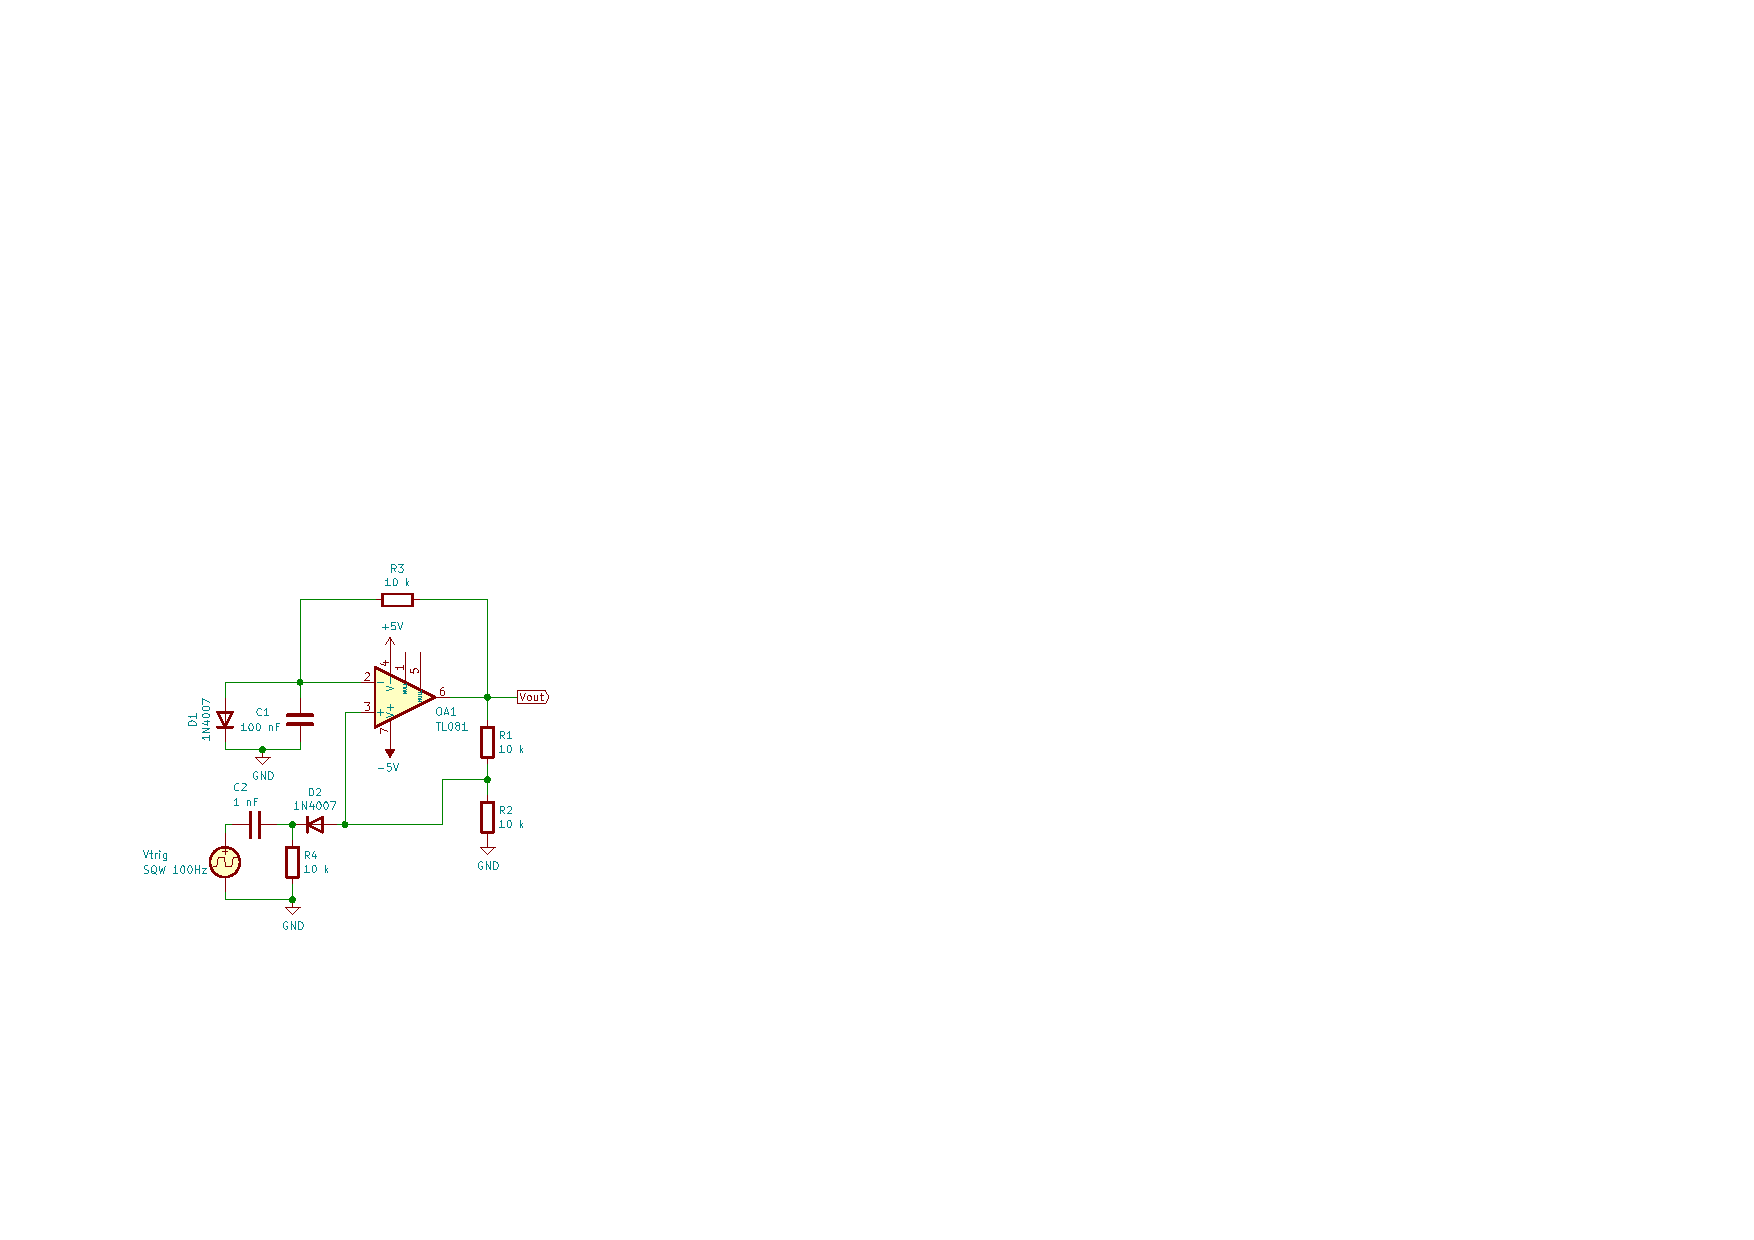
\includegraphics[scale=1.2]{monostable}
    \caption{Schema circuitale del multivibratore monostabile costruito.
    \label{fig: monostableschm}}
\end{figure}

\subsection{Studio dei segnali in ingresso e uscita}
\begin{figure}[htbp]
\centering
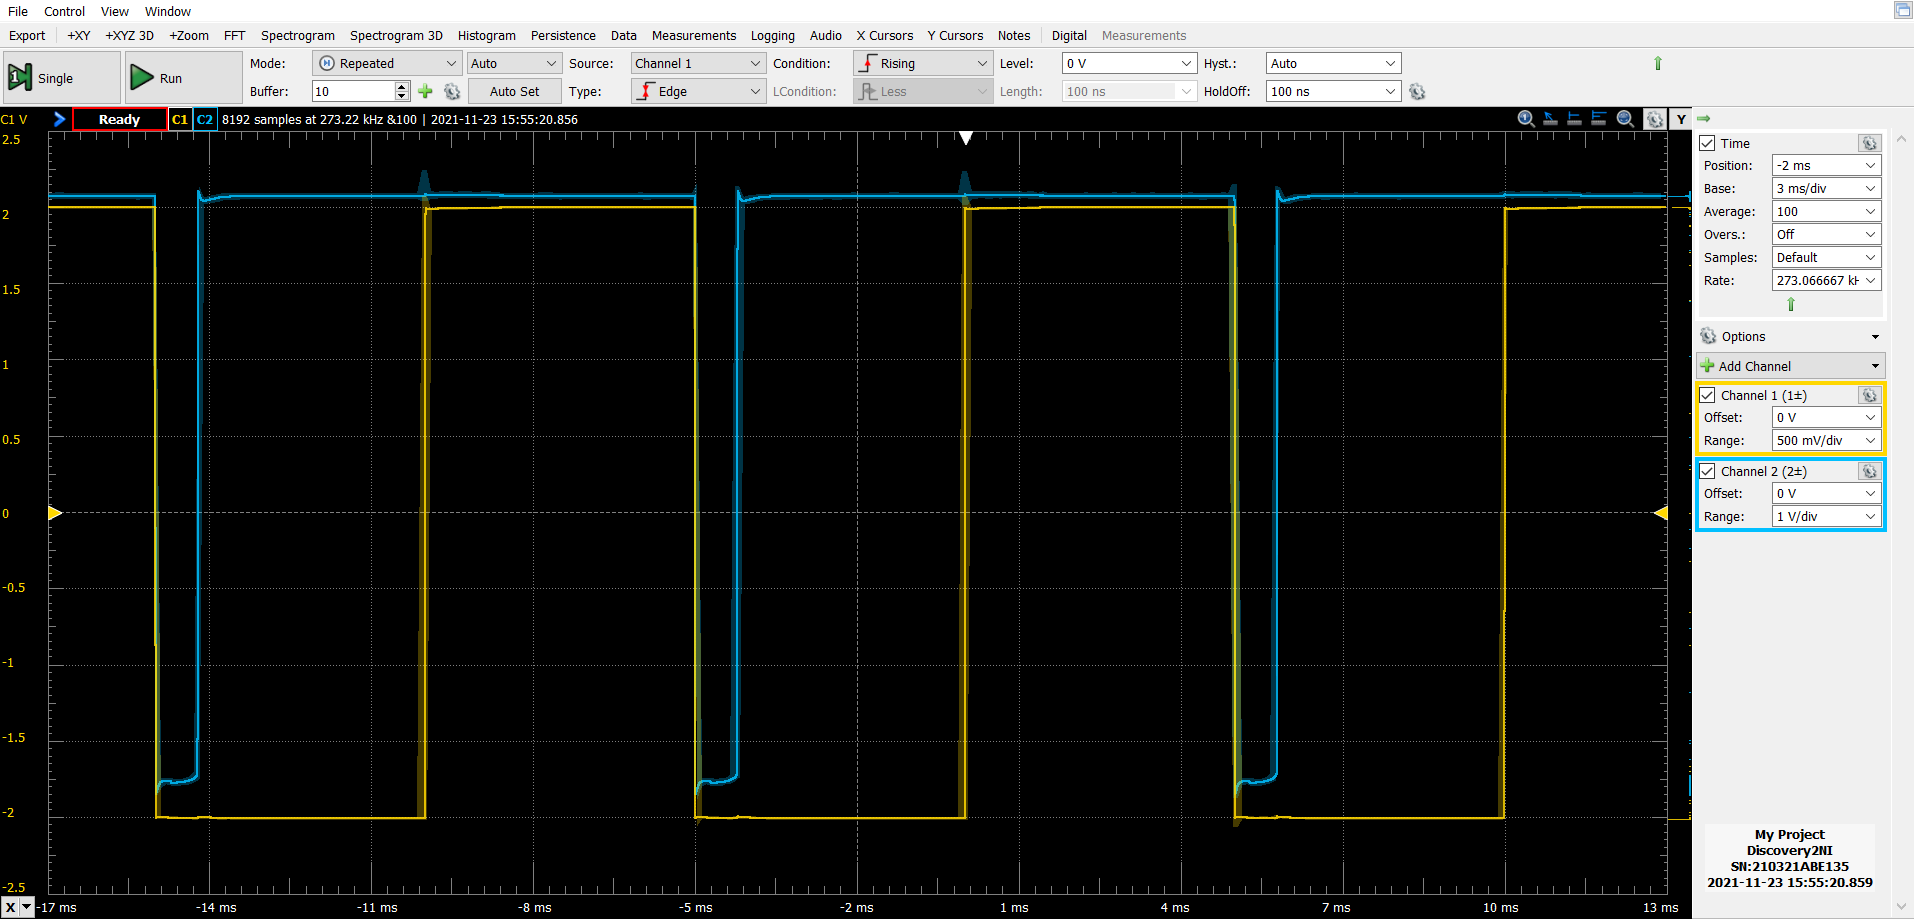
\includegraphics[scale=0.42]{monostabile}
\caption{Grafico segnale in ingresso e $V_{out}$ \label{fig: vout_mstabile}}
\end{figure}

\begin{figure}[htbp]
\centering
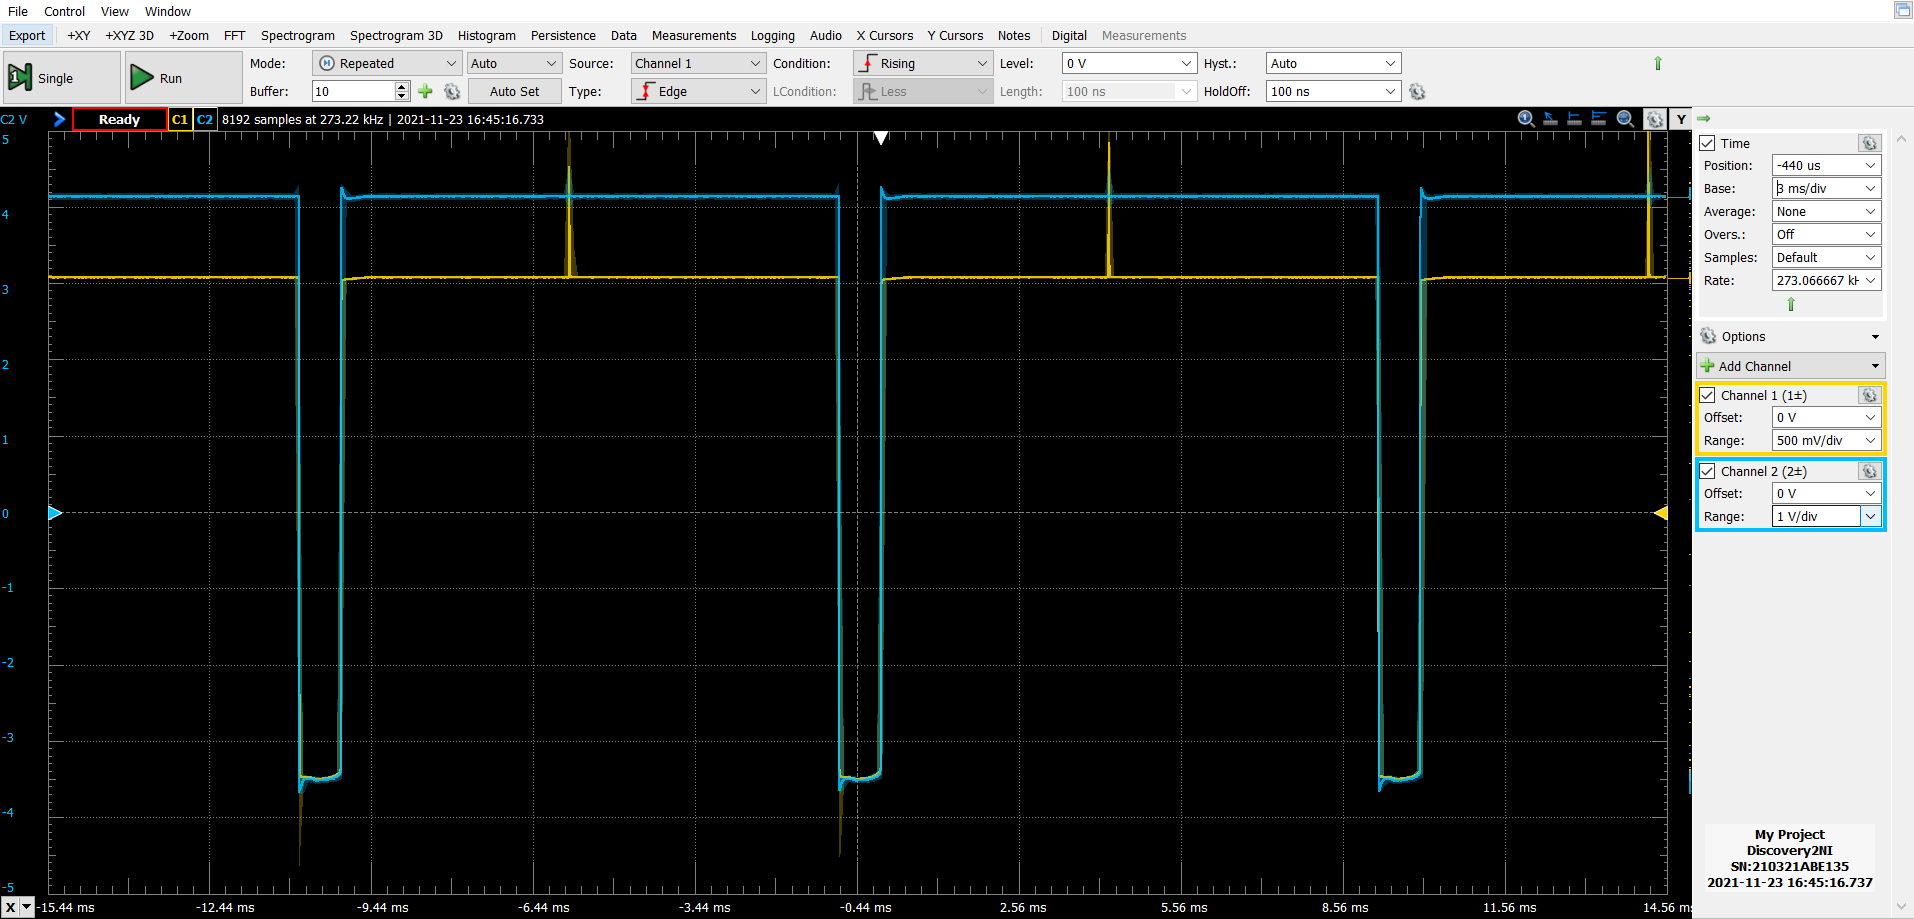
\includegraphics[scale=0.42]{monostabileV+}
\caption{Grafico segnale in $V_+$ e $V_{out}$}
\end{figure}

\begin{figure}[htbp]
\centering
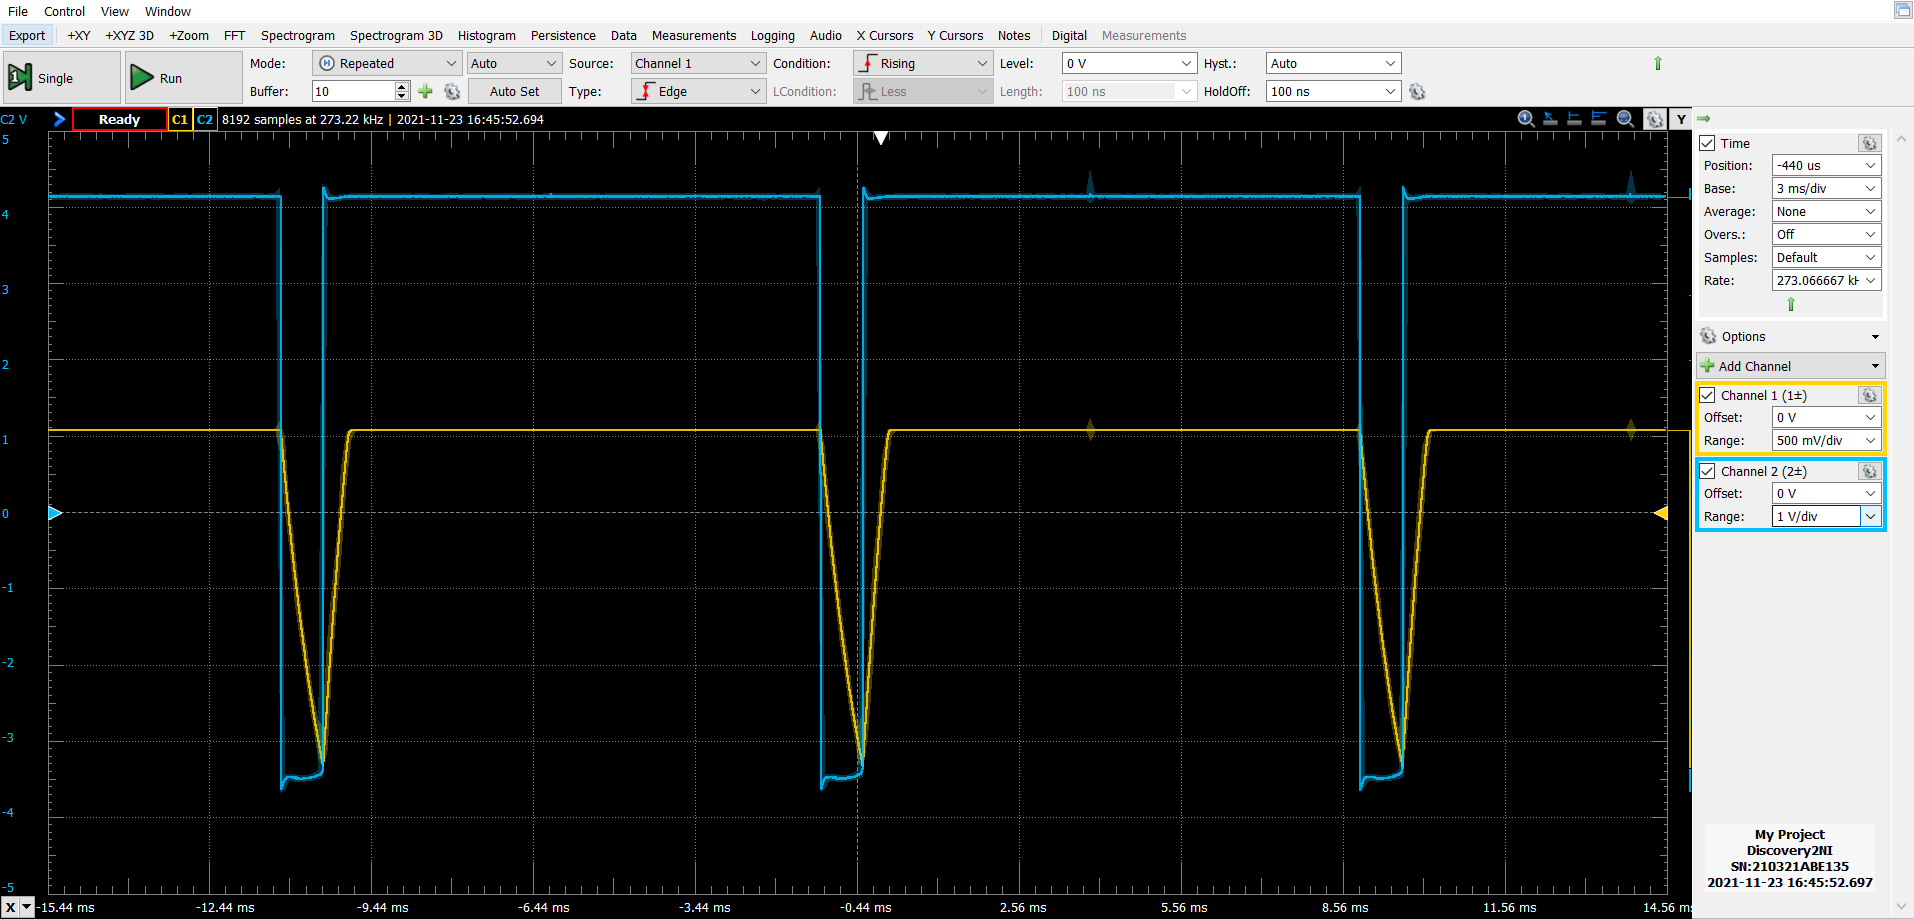
\includegraphics[scale=0.42]{monostabileV-}
\caption{Grafico segnale in $V_-$ e $V_{out}$}
\end{figure}

I segnali osservati riproducono qualitativamente quanto atteso.
In particolare, per $ V \ped{out} $ si osserva un'onda quadra con duty cycle,
per $ V_{-} $ un segnale analogo a $ V\ped{out} $ ma ridotto di un fattore
$\frac{R_2}{R_2 + R_1} \simeq 0.5 $.

Si è misurato il tempo per cui il segnale $ V \ped{out} $ rimane ``basso'' in ogni periodo:

Il valore atteso è
\begin{equation} \label{eq: mstabile}
t\ped{L, exp} =
\tau \log\left[\left(1 + \frac{V_\gamma}{V \ped{out}/2}\right)
\left(1 + \frac{R_2}{R_1}\right)\right]
\end{equation}
riportato senza incertezza data la natura nominale e indicativa del parametro $ V_{\gamma} \simeq \SI{0.7}{\volt} $. Il valore $ \Delta t \ped{exp} $ risulta comparabile con quello misurato.

In assenza del sotto-circuito di trigger, il sistema presenta un solo stato stabile in cui $ V\ped{out} =  V_{\gamma} + V_{z} $.
Come nel caso del multivibratore astabile, $ V\ped{out} $ può assumere solo come valori $ \pm V_{\gamma} + V_{z} $.
Se il condensatore è inizialmente scarico e se è $ V\ped{out} = V_{\gamma} + V_{z} $ allora il condensatore $ C $ si carica fino a quando la caduta ai suoi capi è $ V_{\gamma} $ essendo in parallelo ad un diodo; essendo quindi $ V\ped{+} \sim V_{\gamma} \simeq \SI{0.7}{\volt} $ e $ V_{-} = \frac{R_{2}}{R_{1} + R_{2}} V\ped{out} \simeq 0.5 \times \SI{7}{\volt} = \SI{3.5}{\volt} $, l'uscita rimane ``alta''.
Se il condensatore è inizialmente carico (con caduta ai capi pari a $ V_{\gamma} $) e se è $ V\ped{out} = -(V_{\gamma} + V_{z}) $, allora si scarica fintanto che è $ V_{-} > V_{+} \simeq -\SI{3.5}{\volt} $: a questo, essendo l'OpAmp in regime di saturazione, l'uscita passa a $ V\ped{out} = V_{\gamma} + V_{z} $ e il condensatore si carica come descritto sopra, ripristinando la condizione $ V_{+} \sim V_{\gamma} $. \\

Il sotto-circuito di trigger, formato dal passa-alto con il diodo in cascata, ha la funzione di ``sovrapporre'' a $ V_{+} $ dei picchi di differenza di potenziale negativa che portano il circuito nella configurazione instabile sopra descritta, che, dopo un tempo caratteristico dato dall'equazione~\eqref{eq: mstabile} torna nella configurazione stabile. \\

Come si può vedere in figura~\ref{fig: vout_mstabile}, quanto osservato 
sperimentalmente riproduce qualitativamente l'andamento atteso dall'analisi
teorica del circuito.

\subsection{Durata dell'impulso generato}
\[
V_{S-}= 3.49 \pm 0.03 \si{\V}
\]
\[
V_{OL} = \frac{V_{S-}}{\beta} = 6.95 \pm 0.10 \si{\V}
\]
\[
\Delta= R_3 C_1 \ln(\frac{1 - \frac{V_\gamma}{V_{OL}}}{1 - \beta})= 0.78 \pm 0.03 \si{m\s}
\]
Dalla misura diretta ricavo
\[
\Delta= 779 \pm 10 \;\si{\micro\s}
\]

\subsection{Analisi del funzionamento del circuito}
a discesa di $ V\ped{trig} $ causa l'impulso in $ V\ped{out} $. La risalita in $ V\ped{out} $ accade quando $ V\ped{trig} $ è costante, prima che torni ``alto''. Tale risalita avviene infatti nel momento in cui $ V_{-} $ assume il valore minimo che fa ``scattare'' il discriminatore.

Si tiene fissa l'ampiezza di $ V\ped{trig} $ e se ne varia la frequenza. Si osserva che la durata dell'impulso in $ V \ped{out} $ risulta (entro gli errori di misura) indipendente dalla frequenza del segnale in ingresso, fino a quando la durata di tale impulso è minore del periodo di $ V\ped{trig} $. Al di sopra di tale frequenza critica (sperimentalmente $ f \sim \SI{974}{\hertz} $) il circuito smette di funzionare correttamente.

Si tiene la frequenza di $ V\ped{trig} $ e se ne varia l'ampiezza. La durata dell'impulso in $ V\ped{out} $ risulta (entro gli errori di misura) indipendente dall'ampiezza del segnale in ingresso fintanto $ V\ped{trig} $ è maggiore di una certa soglia. Si osserva sperimentalmente che al di sotto di $ V\ped{trig} \sim \SI{3.7}{\volt} $ il circuito rimane nella configurazione stabile. Infatti se $ V\ped{trig} $ è minore di una certa soglia ci aspettiamo che $ V_{+} $, dato dalla sovrapposizione dell'impulso prodotto dal sotto-circuito di trigger e del segnale uscente dal partitore, non sia abbastanza grande da rendere $ V_{+} - V_{-} $ negativo e far scattare il discriminatore.


%=======================
\section*{Conclusioni e commenti finali}
Si è riusciti a costruire e studiare alcuni dei circuiti più comuni che si
possono realizzare con un amplificatore operazionale, tra cui: due filtri
attivi, passa-basso e passa-alto, un amplificatore di tensione invertente
(e uno non).
In particolare siamo riusciti ad apprezzare il differente comportamento dei
circuiti (anche in regime non lineare) dare una stima di guadagno, impedenza di
ingresso e frequenze caratteristiche della loro risposta in frequenza.

%=======================
\section*{Dichiarazione}
I firmatari di questa relazione dichiarano che il contenuto della relazione \`e
originale, con misure effettuate dai membri del gruppo, e che tutti i firmatari
hanno contribuito alla elaborazione della relazione stessa.

\newpage
\subsection*{Appendice}
Consideriamo il sotto-circuito formato dal condensatore $C_T$ e dal circuito
di formazione. La funzione di trasferimento che lega $V_s$ a $V\ped{sh}$ è
data di fatto da quella di un amplificatore invertente con impedenze
complesse: in trasformata di Laplace
\[
\tilde{A}(s) = - \frac{\left(\frac{1}{R_1} + s 
C_F\right)^{-1}}{\frac{1}{s C_T}} = - \frac{C_T}{C_F} 
\frac{s}{s + \frac{1}{\tau}}
\]
con $ \tau \coloneqq R_1 C_F $. In ingresso abbiamo un'onda quadra di 
periodo $ 2T $ (che prendiamo nulla per tempi negativi) che possiamo scrivere 
come
\[
V\ped{in}(t) = \sum_{k=0}^{+\infty} (-1)^{k}f(t - kT)
\qquad \text{dove} \quad
f(t) = V_s \left[\theta(t) - \theta(t - T)\right]
\]
In trasformata di Laplace si ha
\[
\tilde{f}(s) = V_s\left[\frac{1}{s} - \frac{e^{-sT}}{s}\right]
\]
da cui
\[
\tilde{V}\ped{in}(s) = \sum_{k=0}^{+\infty} (-1)^{k} \tilde{f}(s) e^{-kTs} = 
\tilde{f}(s) \sum_{k=0}^{+\infty} (-1)^{k} e^{-kTs}
\]
La risposta del circuito in trasformata è
\[
  \tilde{V}\ped{sh}(s) = \tilde{A}(s) \tilde{V}\ped{in}(s) =  
\tilde{A}(s)\tilde{f}(s) \sum_{k=0}^{+\infty} (-1)^{k}e^{-kTs} = \tilde{g}(s) 
\sum_{k=0}^{+\infty} (-1)^{k}e^{-kTs} = \mathcal{L}\left[\sum_{k=0}^{+\infty} 
(-1)^{k}g(t - kT)\right](s)
\]
Ora
\[
  \tilde{g}(s) = - V_s \frac{C_T}{C_F} \left[\frac{1}{s + 
\frac{1}{\tau}} - \frac{e^{-sT}}{s + \frac{1}{\tau}}\right]
\]
da cui, anti-trasformando
\[
  g(t) = - V_s \frac{C_T}{C_F} \left[e^{-t/\tau}\theta(t) - 
e^{-(t-T)/\tau} \theta(t - T) \right]
\]

Ma allora la risposta del circuito nel dominio del tempo è
\begin{align*}
  V\ped{sh}(t) &= - V_s \frac{C_T}{C_F} \left\{ 
\sum_{k=0}^{+\infty} (-1)^{k}e^{-\frac{t - kT}{\tau}}\theta(t - kT) - 
\sum_{k=0}^{+\infty} (-1)^{k} e^{-\frac{t- (k+1) T }{\tau}} \theta(t - (k+1)T ) 
\right\} \\
               &= - V_s \frac{C_T}{C_F} \left\{ e^{-\frac{t}{\tau}} 
\theta(t) - 2 \sum_{k=1}^{+\infty} (-1)^{k} e^{-\frac{t - kT}{\tau}} \theta(t - 
kT) \right\}
\end{align*}
ovvero, ignorando il transiente iniziale e supponendo $ \tau\ll T $\footnote{
La buona definizione della somma è assicurata dal fatto che (tralasciando le 
costanti fisiche)
\[ \sum_{k \geq 0} \theta(t-k) e^{-(t-k)} = \sum_{k=0}^{\lfloor t \rfloor} 
e^{-(t-k)} \leq \frac{e}{e-1} e^{-\{t\}}. \]
},
\begin{align}\label{eq:Vshaper}
V\ped{sh}(t) &\approx 2 V_s \frac{C_T}{C_F} \sum_{k=1}^{+\infty} 
(-1)^{k} e^{-\frac{t - kT}{\tau}} \theta(t - kT) \nonumber\\
               &\approx  2 V_s \frac{C_T}{C_F} \sum_{k=1}^{+\infty} 
(-1)^{k} e^{-\frac{t - kT}{\tau}} \chi_{[kT, (k+1)T]}(t)
\end{align}

\end{document}
